
\chapter{Foundation for inference}
\label{FoundationForInference}

\begin{example}{Suppose your professor splits the students in class into two groups: students on the left and students on the right. If $\hat{p}_{_L}$ and $\hat{p}_{_R}$ represent the proportion of students who own an Apple product on the left and right, respectively, would you be surprised if $\hat{p}_{_L}$ did not {exactly} equal $\hat{p}_{_R}$?}\label{classRightLeftSideApple}
While the proportions would probably be close to each other, they are probably not exactly the same. We would probably observe a small difference due to {chance}.
\end{example}

\begin{exercise}
If we don't think the side of the room a person sits on in class is related to whether the person owns an Apple product, what assumption are we making about the relationship between these two variables?\footnote{We would be assuming that these two variables are \emph{independent}, meaning they are unrelated.}
\end{exercise}

Studying randomness of this form is a key focus of statistics. In~this chapter, we'll explore this type of randomness in the context of several applications, and we'll learn new tools and ideas that will be applied throughout the rest of the book.



%_________________
\section{Randomization case study: gender discrimination}
\label{caseStudyGenderDiscrimination}

\index{data!discrimination|(}

We consider a study investigating gender discrimination in the 1970s, which is set in the context of personnel decisions within a bank.\footnote{Rosen B and Jerdee T. 1974. Influence of sex role stereotypes on personnel decisions. Journal of Applied Psychology 59(1):9-14.} The research question we hope to answer~is, ``Are females discriminated against in promotion decisions made by male managers?''

\subsection{Variability within data}
\label{variabilityWithinData}

The participants in this study were 48 male bank supervisors attending a management institute at the University of North Carolina in 1972. They were asked to assume the role of the personnel director of a bank and were given a personnel file to judge whether the person should be promoted to a branch manager position. The files given to the participants were identical, except that half of them indicated the candidate was male and the other half indicated the candidate was female. These files were randomly assigned to the subjects.

\begin{exercise}
Is this an observational study or an experiment? How does the type of study impact what can be inferred from the results?\footnote{The study is an experiment, as subjects were randomly assigned a male file or a female file. Since this is an experiment, the results can be used to evaluate a causal relationship between gender of a candidate and the promotion decision.}
\end{exercise}

For each supervisor we recorded the gender associated with the assigned file and the promotion decision. Using the results of the study summarized in Table~\ref{discriminationResults}, we would like to evaluate if females are unfairly discriminated against in promotion decisions. In this study, a smaller proportion of females are promoted than males (0.583 versus 0.875), but it is unclear whether the difference provides \emph{convincing evidence} that females are unfairly discriminated against.

\begin{table}[ht]
\centering
\begin{tabular}{l l cc rr}
& & \multicolumn{2}{c}{\var{decision}} \\
  \cline{3-4}
		&			& 	{promoted} 	& {not promoted} & Total & \hspace{3mm}  \\ 
  \cline{2-5}
		&	{male} 			& 21    		& 3   & 24  	 \\ 
  \raisebox{1.5ex}[0pt]{\var{gender}}		&	{female} 	& 14    		& 10     & 24	 \\ 
  \cline{2-5}
  		&	Total		& 35	& 13	&  48 \\
  \cline{2-5}
\end{tabular}
\caption{Summary results for the gender discrimination study.}
\label{discriminationResults}
\end{table}

\begin{example}{Statisticians are sometimes called upon to evaluate the strength of evidence. When looking at the rates of promotion for males and females in this study, why might we be tempted to immediately conclude that females are being discriminated against?}\label{discriminationResultsWhatIsConvincingEvidence}
The large difference in promotion rates (58.3\% for females versus 87.5\% for males) suggest there might be discrimination against women in promotion decisions. However, we cannot yet be sure if the observed difference represents discrimination or is just from random chance. Generally there is a little bit of fluctuation in sample data, and we wouldn't expect the sample proportions to be \emph{exactly} equal, even if the truth was that the promotion decisions were independent of gender.
\end{example}

Example~\ref{discriminationResultsWhatIsConvincingEvidence} is a reminder that the observed outcomes in the sample may not perfectly reflect the true relationships between variables in the underlying population. Table~\ref{discriminationResults} shows there were 7 fewer promotions in the female group than in the male group, a difference in promotion rates of 29.2\% $\left( \frac{21}{24} - \frac{14}{24} = 0.292 \right)$. This observed difference is what we call a \term{point estimate} of the true effect. The point estimate of the difference is large, but the sample size for the study is small, making it unclear if this observed difference represents discrimination or whether it is simply due to chance. We label these two competing claims, $H_0$ and $H_A$:
\begin{itemize}
\setlength{\itemsep}{0mm}
\item[$H_0$:] \textbf{Null hypothesis.} The variables \var{gender} and \var{decision} are independent. They have no relationship, and the observed difference between the proportion of males and females who were promoted, 29.2\%, was due to chance.
\item[$H_A$:] \textbf{Alternative hypothesis.} The variables \var{gender} and \var{decision} are \emph{not} independent. The difference in promotion rates of 29.2\% was not due to chance, and equally qualified females are less likely to be promoted than males.
\end{itemize}

\begin{termBox}{\tBoxTitle{Hypothesis testing}
These hypotheses are part of what is called a \term{hypothesis test}. A hypothesis test is a statistical technique used to evaluate competing claims using data. Often times, the null hypothesis takes a stance of \emph{no difference} or \emph{no effect}. If the null hypothesis and the data notably disagree, then we will reject the null hypothesis in favor of the alternative hypothesis. \vspace{3mm}

Don't worry if you aren't a master of hypothesis testing at the end of this section. We'll discuss these ideas and details many times in this chapter, most notably in Section~\ref{HypothesisTesting}.}
\end{termBox}

What would it mean if the null hypothesis, which says the variables \var{gender} and \var{decision} are unrelated, is true? It would mean each banker would decide whether to promote the candidate without regard to the gender indicated on the file. That~is, the difference in the promotion percentages would be due to the way the files were randomly divided to the bankers, and the randomization just happened to give rise to a relatively large difference of 29.2\%.

Consider the alternative hypothesis: bankers were influenced by which gender was listed on the personnel file. If this was true, and especially if this influence was substantial, we would expect to see some difference in the promotion rates of male and female candidates. If this gender bias was against females, we would expect a smaller fraction of promotion recommendations for female personnel files relative to the male files.

We will choose between these two competing claims by assessing if the data conflict so much with $H_0$ that the null hypothesis cannot be deemed reasonable. If this is the case, and the data support $H_A$, then we will reject the notion of independence and conclude that these data provide strong evidence of discrimination.

\subsection{Simulating the study}
\label{simulatingTheStudy}

Table~\ref{discriminationResults} shows that 35 bank supervisors recommended promotion and 13 did not. Now, suppose the banker's decisions were independent of gender. Then, if we conducted the experiment again with a different random assignment of files, differences in promotion rates would be based only on random fluctuation. We can actually perform this \term{randomization}, which simulates what would have happened if the bankers' decisions had been independent of gender but we had distributed the files differently.\footnote{The test procedure we employ in this section is formally called a \term{permutation test}.}

In this \term{simulation}, we thoroughly shuffle 48 personnel files, 24 labeled \resp{male} and 24 labeled \resp{female}, and deal these files into two stacks. We will deal 35 files into the first stack, which will represent the 35 supervisors who recommended promotion. The second stack will have 13 files, and it will represent the 13 supervisors who recommended against promotion. Then, as we did with the original data, we tabulate the results and determine the fraction of \resp{male} and \resp{female} who were promoted.

Since the randomization of files in this simulation is independent of the promotion decisions, any difference in the two fractions is entirely due to chance. Table~\ref{discriminationRand1} show the results of such a simulation.

\begin{table}[ht]
\centering
\begin{tabular}{l l cc rr}
& & \multicolumn{2}{c}{\var{decision}} \\
  \cline{3-4}
		&			& 	{promoted} 	& {not promoted} & Total & \hspace{3mm}  \\ 
  \cline{2-5}
		&	male 					& 18    		& 6    & 24 	 \\ 
  \raisebox{1.5ex}[0pt]{\var{gender\_\hspace{0.3mm}simulated}}		&	female 	& 17    		& 7 & 24    	 \\ 
  \cline{2-5}
  & Total	& 35 & 13 & 48
\end{tabular}
\caption{Simulation results, where any difference in promotion rates between \resp{male} and \resp{female} is purely due to chance.}
\label{discriminationRand1}
\end{table}

\textPE{\pagebreak}

\begin{exercise} \label{sampleDifferenceInMaleAndFemaleDiscrimination}
What is the difference in promotion rates between the two simulated groups in Table~\ref{discriminationRand1}? How does this compare to the observed difference 29.2\% from the actual~study?\footnote{$18/24 - 17/24=0.042$ or about 4.2\% in favor of the men. This difference due to chance is much smaller than the difference observed in the actual groups.}
\end{exercise}

\subsection{Checking for independence}

We computed one possible difference under the null hypothesis in Exercise~\ref{sampleDifferenceInMaleAndFemaleDiscrimination}, which represents one difference due to chance. While in this first simulation, we physically dealt out files, it is much more efficient to perform this simulation using a computer. Repeating the simulation on a computer, we get another difference due to chance: -0.042. And another: 0.208. And so on until we repeat the simulation enough times that we have a good idea of what represents the \emph{distribution of differences from chance alone}. Figure~\ref{discRandDotPlot} shows a plot of the differences found from 100 simulations, where each dot represents a simulated difference between the proportions of male and female files recommended for promotion.

\begin{figure}[ht]
\centering
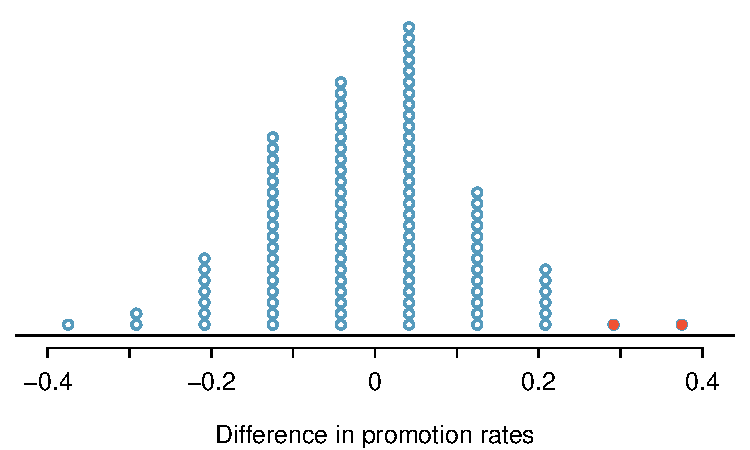
\includegraphics[width=0.7\textwidth]{02/figures/discRandDotPlot/discRandDotPlot}
\caption{A stacked dot plot of differences from 100 simulations produced under the null hypothesis, $H_0$, where \var{gender\_\hspace{0.3mm}simulated} and \var{decision} are independent. Two of the 100 simulations had a difference of at least 29.2\%, the difference observed in the study, and are shown as solid dots.}
\label{discRandDotPlot}
\end{figure}

Note that the distribution of these simulated differences is centered around 0. Because we simulated differences in a way that made no distinction between men and women, this makes sense: we should expect differences from chance alone to fall around zero with some random fluctuation for each simulation.

\begin{example}{How often would you observe a difference of at least 29.2\% (0.292) according to Figure~\ref{discRandDotPlot}? Often, sometimes, rarely, or never?}
It appears that a difference of at least 29.2\% due to chance alone would only happen about 2\% of the time according to Figure~\ref{discRandDotPlot}. Such a low probability indicates that observing such a large difference from chance is rare.
\end{example}

The difference of 29.2\% is a rare event if there really is no impact from listing gender in the candidates' files, which provides us with two possible interpretations of the study results:
\begin{itemize}
\setlength{\itemsep}{0mm}
\item[$H_0$:] \textbf{Null hypothesis.} Gender has no effect on promotion decision, and we observed a difference that would only happen rarely.
\item[$H_A$:] \textbf{Alternative hypothesis.} Gender has an effect on promotion decision, and what we observed was actually due to equally qualified women being discriminated against in promotion decisions, which explains the large difference of 29.2\%.
\end{itemize}
When we conduct formal studies, we reject a skeptical position if the data strongly conflict with that position.%When we conduct formal studies, usually we reject the notion that we just happened to observe a rare event.
\footnote{This reasoning does not generally extend to anecdotal observations. Each of us observes incredibly rare events every day, events we could not possibly hope to predict. However, in the non-rigorous setting of anecdotal evidence, almost anything may appear to be a rare event, so the idea of looking for rare events in day-to-day activities is treacherous. For example, we might look at the lottery: there was only a 1 in 176 million chance that the Mega Millions numbers for the largest jackpot in history (March 30, 2012) would be (2, 4, 23, 38, 46) with a Mega ball of (23), but nonetheless those numbers came up! However, no matter what numbers had turned up, they would have had the same incredibly rare odds. That is, \emph{any set of numbers we could have observed would ultimately be incredibly rare}. This type of situation is typical of our daily lives: each possible event in itself seems incredibly rare, but if we consider every alternative, those outcomes are also incredibly rare. We should be cautious not to misinterpret such anecdotal evidence.} 
%In this case, we reject the null hypothesis in favor of the alternative. 
In our analysis, we determined that there was only a $\approx$2\% probability of obtaining a sample where $\geq$29.2\% more males than females get promoted by chance alone, so we conclude the data provide strong evidence of gender discrimination against women by the supervisors. In this case, we reject the null hypothesis in favor of the alternative.

\index{data!discrimination|)}

Statistical inference is the practice of making decisions and conclusions from data in the context of uncertainty. Errors do occur, just like rare events, and the data set at hand might lead us to the wrong conclusion. While a given data set may not always lead us to a correct conclusion, statistical inference gives us tools to control and evaluate how often these errors occur. Before getting into the nuances of hypothesis testing, let's work through another case study.


%_________________
%\section{Case study: stents and strokes [2 prop randomization]}

\textPE{\newpage}

%_________________
\section{Randomization case study: opportunity cost}
\label{caseStudyOpportunityCost}

How rational and consistent is the behavior of the typical American college student? In~this section, we'll explore whether college student consumers always consider an obvious fact: money not spent now can be spent later.

In particular, we are interested in whether reminding students about this well-known fact about money causes them to be a little thriftier. A skeptic might think that such a reminder would have no impact. We can summarize these two perspectives using the null and alternative hypothesis framework.
\begin{itemize}
\setlength{\itemsep}{0mm}
\item[$H_0$:] \textbf{Null hypothesis.} Reminding students that they can save money for later purchases will not have any impact on students' spending decisions.
\item[$H_A$:] \textbf{Alternative hypothesis.} Reminding students that they can save money for later purchases will reduce the chance they will continue with a purchase.
\end{itemize}
In this section, we'll explore an experiment conducted by researchers that investigates this very question for students at a university in the southwestern United States.\footnote{Frederick S, Novemsky N, Wang J, Dhar R, Nowlis S. 2009. Opportunity Cost Neglect. Journal of Consumer Research 36: 553-561.}

\subsection{Exploring the data set before the analysis}

%Shane Frederick of Yale School of Management and his collaborators conducted an experiment exploring the rational behavior of consumers. 
One-hundred and fifty students were recruited for the study, and each was given the following statement:
\begin{quote}
% Suppose when a person is about to spend money, we simply reminded them that they could spend the money on something else. Would it have any impact on the likelihood that they would continue with the purchase?
%What would you do in this situation? Please circle one of the options below.
Imagine that you have been saving some extra money on the side to make some purchases, and on your most recent visit to the video store you come across a special sale on a new video. This video is one with your favorite actor or actress, and your favorite type of movie (such as a comedy, drama, thriller, etc.). This particular video that you are considering is one you have been thinking about buying for a long time. It is available for a special sale price of \$14.99.

What would you do in this situation? Please circle one of the options below.
\end{quote}
Half of the 150 students were randomized into a control group and were given the following two options:
\begin{quote}
(A) Buy this entertaining video.

(B) Not buy this entertaining video.
\end{quote}
The remaining 75 students were placed in the treatment group, and they saw a slightly modified option (B):
\begin{quote}
(A) Buy this entertaining video.

(B) Not buy this entertaining video. Keep the \$14.99 for other purchases.
\end{quote}
Would the extra statement reminding students of an obvious fact impact the purchasing decision? Table~\ref{OpportunityCostTable} summarizes the study results.

\begin{table}[ht]
\centering
\begin{tabular}{l cc rr}
& \multicolumn{2}{c}{decision} \\
\cline{2-3}
				& {buy DVD}\ \  	& {not buy DVD} & Total & \hspace{3mm}  \\ 
\cline{1-4}
control group 		& 56		& 19	& 75 \\ 
treatment group 	& 41		& 34	& 75 \\ 
\cline{1-4}
Total				& 97		& 53	& 150
\end{tabular}
\caption{Summary of student choices in the opportunity cost study.}
%150 participants were asked whether they would buy a DVD under a particular circumstance. Participants in the control group were given two options, and participants in the treatment group were given the same options, except in the \emph{not buy} option they were reminded that not spending the money meant the money could be used for a later purchase. This table summarizes the results from the study.}
\label{OpportunityCostTable}
\end{table}

It might be a little easier to review the results using row proportions, specifically considering the proportion of participants in each group who said they would buy or not buy the DVD. These summaries are given in Table~\ref{OpportunityCostTableRowProp}.

\begin{table}[ht]
\centering
\begin{tabular}{l cc rr}
& \multicolumn{2}{c}{decision} \\
\cline{2-3}
				& {buy DVD}\ \  	& {not buy DVD} & Total & \hspace{3mm}  \\ 
\cline{1-4}
control group 		& 0.747	& 0.253	& 1.000 \\ 
treatment group 	& 0.547	& 0.453	& 1.000 \\ 
\cline{1-4}
Total				& 0.647	& 0.353	& 1.000
\end{tabular}
\caption{The data from Table~\ref{OpportunityCostTable} summarized using row proportions. Row proportions are particularly useful here since we can view the proportion of \emph{buy} and \emph{not buy} decisions in each group.}
\label{OpportunityCostTableRowProp}
\end{table}

We will define a \term{success} in this study as a student who chooses not to buy the DVD.\footnote{Success is often defined in a study as the outcome of interest, and a ``success'' may or may not actually be a positive outcome. For example, researchers working on a study on HIV prevalence might define a ``success'' in the statistical sense as a patient who is HIV+. A more complete discussion of the term \emph{success} will be given in Chapter~\ref{inferenceForCategoricalData}. } Then, the value of interest is the change in DVD purchase rates that results by reminding students that not spending money now means they can spend the money later.
%A first look at the data suggests that reminding students that not spending money means they can spend the money later has an impact. 
We can construct a point estimate for this difference as
\begin{align*}
\hat{p}_{trmt} - \hat{p}_{ctrl}
  = \frac{34}{75} - \frac{19}{75}
  = 0.453 - 0.253
  = 0.200
\end{align*}
The proportion of students who chose not to buy the DVD was 20\% higher in the treatment group than the control group.
However, is this result \term{statistically significant}? In~other words, is a 20\% difference so prominent that it is unlikely to have occurred from chance~alone?

\subsection{Results from chance alone}

The primary goal in this data analysis is to understand what sort of differences we might see if the null hypothesis were true, i.e. the treatment had no effect on students. For this, we'll use the same procedure we applied in Section~\ref{caseStudyGenderDiscrimination}: randomization.

Let's think about the data in the context of the hypotheses. If the null  hypothesis~($H_0$) was true and the treatment had no impact on student decisions, then the observed difference between the two groups of 20\% could be attributed entirely to chance. If,~on the other hand, the alternative hypothesis ($H_A$) is true, then the difference indicates that reminding students about saving for later purchases actually impacts their buying decisions.

Just like with the gender discrimination study, we can perform a statistical analysis. Using the same randomization technique from the last section, let's see what happens when we simulate the experiment under the scenario where there is no effect from the treatment.

While we would in reality do this simulation on a computer, it might be useful to think about how we would go about carrying out the simulation without a computer. We~start with 150 index cards and label each card to indicate the distribution of our response variable: decision. That is, 53 cards will be labeled ``not buy DVD'' to represent the 53 students who opted not to buy, and 97 will be labeled ``buy DVD'' for the other 97 students. Then we shuffle these cards throughly and divide them into two stacks of size 75, representing the simulated treatment and control groups. Any observed difference between the proportions of ``not buy DVD'' cards (what we earlier defined as \emph{success}) can be attributed entirely to chance.

\begin{example}{If we are randomly assigning the cards into the simulated treatment and control groups, how many ``not buy DVD'' cards would we expect to end up with in each simulated group? What would be the expected difference between the proportions of ``not buy DVD'' cards in each group?}
Answer: Since the simulated groups are of equal size, we would expect $53 / 2 = 26.5$, i.e. 26 or 27, ``not buy DVD'' cards in each simulated group, yielding a simulated point estimate of 0\%. However, due to random fluctuations, we might actually observe a number a little above or below 26 and 27.
\end{example}

%We'll take the students and randomize them into two new groups, simulated-control and simulated-treatment groups, and then we'll look at the difference in the two groups. 
The results of a randomization from chance alone is shown in Table~\ref{OpportunityCostTableSimulated}. From this table, we can compute a difference that occurred from chance~alone:
\begin{align*}
\hat{p}_{trmt, simulated} - \hat{p}_{ctrl, simulated}
  = \frac{24}{75} - \frac{29}{75}
  = 0.32 - 0.387
  = - 0.067
\end{align*}
%This difference of -6.7\% is entirely due to chance.

\begin{table}[ht]
\centering
\begin{tabular}{l cc rr}
& \multicolumn{2}{c}{decision} \\
\cline{2-3}
				& {buy DVD}\ \  	& {not buy DVD} & Total & \hspace{3mm}  \\ 
\cline{1-4}
simulated-control group 		& 46		& 29	& 75 \\ 
simulated-treatment group 	& 51		& 24	& 75 \\ 
\cline{1-4}
Total				& 97		& 53	& 150
\end{tabular}
\caption{Summary of student choices against their simulated groups. The group assignment had no connection to the student decisions, so any difference between the two groups is due to chance.}
\label{OpportunityCostTableSimulated}
\end{table}

Just one simulation will not be enough to get a sense of what sorts of differences would happen from chance alone. We'll simulate another set of simulated groups and compute the new difference: 0.013. And again: 0.067. And again: -0.173. We'll do this 1,000 times. The results are summarized in a dot plot in Figure~\ref{OpportunityCostDiffsDotPlot}, where each point represents a simulation. Since there are so many points, it is more convenient to summarize the results in a histogram such as the one in Figure~\ref{OpportunityCostDiffs}, where the height of each histogram bar represents the fraction of observations in that group.

\begin{figure}[ht]
\centering
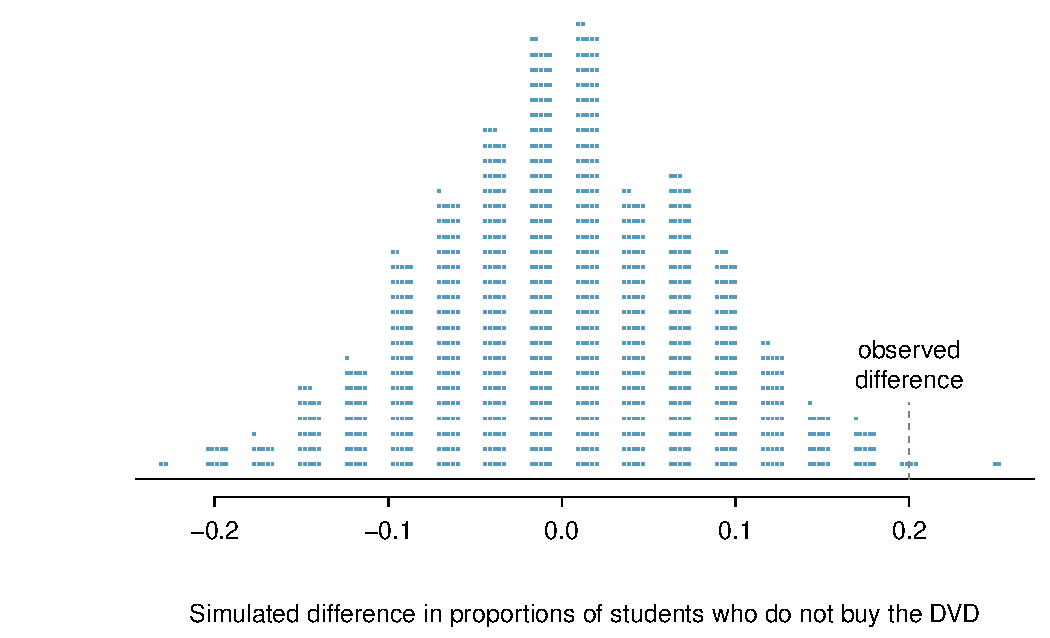
\includegraphics[width=0.95\textwidth]{02/figures/OpportunityCost/OpportunityCostDiffsDotPlot}
\caption{A stacked dot plot of 1,000 chance differences produced under the null hypothesis, $H_0$. Six of the 1,000 simulations had a difference of at least 20\%, which was the difference observed in the study.}
\label{OpportunityCostDiffsDotPlot}
\end{figure}

\begin{figure}[ht]
\centering
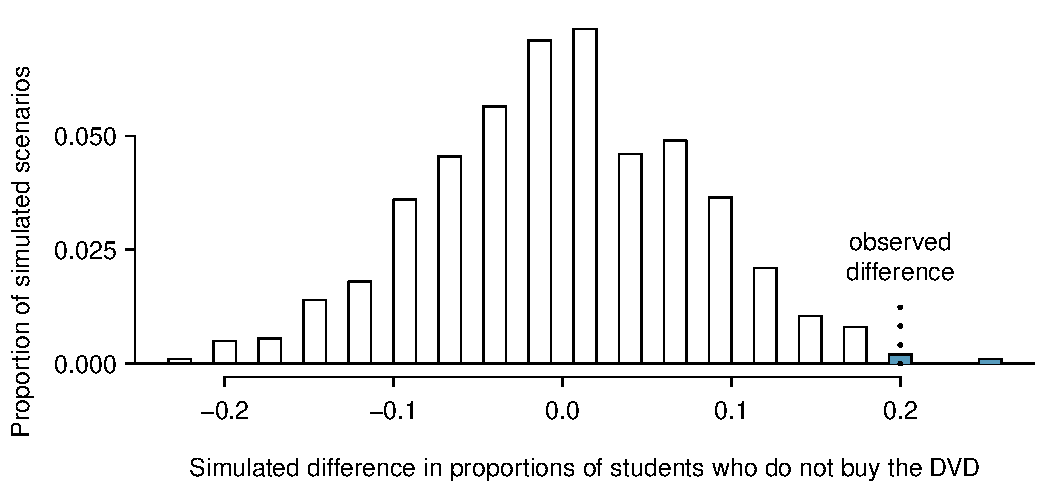
\includegraphics[width=0.95\textwidth]{02/figures/OpportunityCost/OpportunityCostDiffsRightTail}
\caption{A histogram of 1,000 chance differences produced under the null hypothesis, $H_0$. Six of the 1,000 simulations had a difference of at least 20\%, which was the difference observed in the study.}
\label{OpportunityCostDiffs}
\end{figure}

If there was no treatment effect, then we'd only observe a difference of at least +20\% about 0.6\% of the time, or about 1-in-150 times. That is really rare! Instead, we will conclude the data provide strong evidence there is a treatment effect: reminding students before a purchase that they could instead spend the money later on something else lowers the chance that they will continue with the purchase. Notice that we are able to make a causal statement for this study since the study is an experiment.

%\begin{termBox}{\tBoxTitle{Become a savvy consumer}
%Apply what you just learned by signing a pledge saying that you will be a thoughtful consumer before you make a purchase. Visit \href{http://www.openintro.org/savvyconsumer}{openintro.org/savvyconsumer}.}
%\end{termBox}

%\Comment{Scrap box above? Or would it be fun? If keep, TODO(David): build a webpage for openintro.org/savvyconsumer.}



% conducted the study again with the same students. If the treatment had no influence on their decisions, each student would respond the same. We would still have 97 students would would buy the DVD and 53 students who would not. If we randomly split these students up into the treatment and control groups, we are simulating what might have happened if (1) we could repeat the study and (2) the null hypothesis was true, meaning the treatment has no effect.

%Table~\ref{} represents a new randomization of students into the treatment and control groups. In this simulation, we see that the 




%What if we could encourage more thoughtful spending by consumers by pointing out the obvious fact that they could spend money on different things? This was the 
%
%Capitalism is built on the premise that individuals make rational decision. What if we could 
%
%What if we told you there was a simple way to make people more thoughtful about how they spend their money?
%
%If shoppers are reminded that if they don't spend money today, they can spend it tomorrow, do you think that would have an influence on their shopping behavior?
%
%Consider the following scenario, which was given to 150 students:
%\begin{quote}
%Imagine that you have been saving some extra money on the side to make some purchases, and on your most recent visit to the video store you come across a special sale on a new video. This video is one with your favorite actor or actress, and your favorite type of movie (such as a comedy, drama, thriller, etc.). This particular video that you are considering is one you have been thinking about buying for a long time. It is available for a special sale price of \$14.99.
%\end{quote}





%_________________
\section{Hypothesis testing}
\label{HypothesisTesting}

In the last two sections, we utilized a \term{hypothesis test}, which is a formal technique for evaluating two competing possibilities. In each scenario, we described a \term{null hypothesis}, which represented either a skeptical perspective or a perspective of no difference. We also laid out an \term{alternative hypothesis}, which represented a new perspective such as the possibility that there has been a change or that there is a treatment effect in an experiment.

\begin{termBox}{\tBoxTitle{Null and alternative hypotheses}
The \term{null hypothesis ($H_0$)} often represents either a skeptical perspective or a claim to be tested. The \term{alternative hypothesis ($H_A$)} represents an alternative claim under consideration and is often represented by a range of possible values for the value of~interest.}
\end{termBox}

The hypothesis testing framework is a very general tool, and we often use it without a second thought. If a person makes a somewhat unbelievable claim, we are initially skeptical. However, if there is sufficient evidence that supports the claim, we set aside our skepticism. The hallmarks of hypothesis testing are also found in the US court system. 

\subsection{Hypothesis testing in the US court system}

\begin{example}{A US court considers two possible claims about a defendant: she is either innocent or guilty. If we set these claims up in a hypothesis framework, which would be the null hypothesis and which the alternative?}\label{hypTestCourtExample}
The jury considers whether the evidence is so convincing (strong) that there is no reasonable doubt regarding the person's guilt. That is, the skeptical perspective (null hypothesis) is that the person is innocent until evidence is presented that convinces the jury that the person is guilty (alternative hypothesis).
\end{example}

Jurors examine the evidence to see whether it convincingly shows a defendant is guilty. Notice that if a jury finds a defendant \emph{not guilty}, this does not necessarily mean the jury is confident in the person's innocence. They are simply not convinced of the alternative that the person is guilty.

This is also the case with hypothesis testing: \emph{even if we fail to reject the null hypothesis, we typically do not accept the null hypothesis as truth}. Failing to find strong evidence for the alternative hypothesis is not equivalent to providing evidence that the null hypothesis is true.

%\begin{tipBox}{\tipBoxTitle{We never accept the null hypothesis}
%Statistics trains us to keep an }
%\end{tipBox}

\subsection{p-value and statistical significance} %Revisiting the gender discrimination case study}

In Section~\ref{caseStudyGenderDiscrimination} we encountered a study from the 1970's that explored whether there was strong evidence that women were less likely to be promoted than men. The research question -- are females discriminated against in promotion decisions made by male managers? -- was framed in the context of hypotheses:
\begin{itemize}
\setlength{\itemsep}{0mm}
\item[$H_0$:] Gender has no effect on promotion decisions.
\item[$H_A$:] Women are discriminated against in promotion decisions.
\end{itemize}
The null hypothesis ($H_0$) was a perspective of no difference. The data, summarized on page~\pageref{discriminationResults}, provided a point estimate of a 29.2\% difference in recommended promotion rates between men and women. We determined that such a difference from chance alone would be rare: it would only happen about 2 in 100 times. When results like these are inconsistent with $H_0$, we reject $H_0$ in favor of $H_A$. Here, we concluded there was discrimination against women.

The 2-in-100 chance is what we call a \term{p-value}, which is a probability quantifying the strength of the evidence against the null hypothesis and in favor of the alternative. %Formally the p-value is a conditional probability, which is basically\footnote{Want to learn more probability? Check out~Appendix~\ref{probability}.}

\begin{termBox}{\tBoxTitle{p-value}
The \term{p-value}\index{hypothesis testing!p-value|textbf} is the probability of observing data at least as favorable to the alternative hypothesis as our current data set, if the null hypothesis were true. We~typically use a summary statistic of the data to help compute the p-value and evaluate the~hypotheses. This summary value used to compute the p-value is often called the \term{test statistic}.}
\end{termBox}

\begin{example}{In the gender discrimination study, the difference in discrimination rates was our test statistic. What was the test statistic in the opportunity cost study?}
The test statistic in the opportunity cost study was the difference in the proportion of students who decided against the DVD purchase in the treatment and control groups. In each of these examples, the \hiddenterm{point estimate} of the values of interest (the difference in proportions) were  also used as the test statistics.
\end{example}

When the p-value is small, i.e. less than a previously set threshold, we say the results are \term{statistically significant}. This means the data provide such strong evidence against $H_0$ that we reject the null hypothesis in favor of the alternative hypothesis. This threshold, called the \term{significance level}\index{hypothesis testing!significance level}\index{significance level} (often represented by $\alpha$, the Greek letter \emph{alpha}\label{alphadiscussion})\marginpar[\raggedright\vspace{-4mm}

$\alpha$\\\footnotesize significance\\level of a\\hypothesis test]{\raggedright\vspace{-4mm}

$\alpha$\\\footnotesize significance\\level of a\\hypothesis test}, is typically set to $\alpha = 0.05$, but can vary depending on the field or the application. For example, in the discrimination study, we can say that the data provided statistically significant evidence against the null hypothesis.

\begin{termBox}{\tBoxTitle{Statistical significance}
We say that the data provide \term{statistically significant}\index{hypothesis testing!statistically significant|textbf} evidence against the null hypothesis if the p-value is less than some reference value, usually~$\alpha=0.05$.}
\end{termBox}

%\begin{termBox}{\tBoxTitle{Significance Level}
%If the null hypothesis is true, the significance level $\alpha$ defines the probability that we will make a Type~1 Error.}
%\end{termBox}

\begin{example}{In the opportunity cost study in Section~\ref{caseStudyOpportunityCost}, we analyzed an experiment where study participants were 20\% less likely to continue with a DVD purchase if they were reminded that the money, if not spent on the DVD, could be used for other purchases in the future. We determined that such a large difference would only occur about 1-in-150 times if the reminder actually had no influence on student decision-making. What is the p-value in this study? Was the result statistically significant?}
The p-value is the 1-in-150, i.e. 0.007. Since the p-value is less than 0.05, the data provide statistically significant evidence that US college students were actually influenced by the reminder.
\end{example}

\begin{termBox}{\tBoxTitle{What's so special about 0.05?}
We often use a threshold of 0.05 to determine whether a result is statistically significant. But why 0.05? Maybe we should use a bigger number, or maybe a smaller number. If you're a little puzzled, that probably means you're reading with a critical eye -- good job! We've made a video to help clarify \emph{why 0.05}:
\begin{center}
\href{http://www.openintro.org/why05}{www.openintro.org/why05}
\end{center}
Sometimes it's also a good idea to deviate from the standard. We'll discuss when to choose a threshold different than 0.05 in Section~\ref{significanceLevel}.\vspace{0.5mm}}
\end{termBox}

\Comment{TODO(David and/or Shannon): make video!}
% Why is it the rule of thumb rather than a smaller value like 0.010.15 0.01?

%\begin{example}{}

%\end{example}


\subsection{Decision errors}

\index{hypothesis testing!decision errors|(}

Hypothesis tests are not flawless. Just think of the court system: innocent people are sometimes wrongly convicted and the guilty sometimes walk free. Similarly, data can point to the wrong conclusion. However, what distinguishes statistical hypothesis tests from a court system is that our framework allows us to quantify how often the data lead us to the incorrect conclusion.

There are two competing hypotheses: the null and the alternative. In a hypothesis test, we make a statement about which one might be true, but we might choose incorrectly. There are four possible scenarios in a hypothesis test, which are summarized in Table~\ref{fourHTScenarios}.

\begin{table}[ht]
\centering
\begin{tabular}{l l c c}
& & \multicolumn{2}{c}{\textbf{Test conclusion}} \\
  \cline{3-4}
\vspace{-3.7mm} \\
& & do not reject $H_0$ &  reject $H_0$ in favor of $H_A$ \\
  \cline{2-4}
\vspace{-3.7mm} \\
& $H_0$ true & okay &  Type~1 Error \\
\raisebox{1.5ex}{\textbf{Truth}} & $H_A$ true & Type 2 Error & okay \\
  \cline{2-4}
\end{tabular}
\caption{Four different scenarios for hypothesis tests.}
\label{fourHTScenarios}
\end{table}

A \term{Type~1 Error} is rejecting the null hypothesis when $H_0$ is actually true. Since we rejected the null hypothesis in the gender discrimination and opportunity cost studies, it is possible that we made a Type~1 Error in one or both of those studies. A \term{Type~2 Error} is failing to reject the null hypothesis when the alternative is actually true.

\begin{example}{In a US court, the defendant is either innocent ($H_0$) or  guilty ($H_A$). What does a Type~1 Error represent in this context? What does a Type 2 Error represent? Table~\ref{fourHTScenarios} may be useful.}
If the court makes a Type~1 Error, this means the defendant is innocent ($H_0$ true) but wrongly convicted. A Type 2 Error means the court failed to reject $H_0$ (i.e. failed to convict the person) when she was in fact guilty ($H_A$ true).
\end{example}

\begin{exercise}
Consider the opportunity cost study where we concluded students were less likely to make a DVD purchase if they were reminded that money not spent now could be spent later. What would a Type~1 Error represent in this context?\footnote{A Type~1 Error would mean that we incorrectly rejected $H_0$, where the null hypothesis in this case was that the observed difference was due to chance. Notice that this does \emph{not} necessarily mean something was wrong with the data or that we made a computational mistake. Sometimes data simply point us to the wrong conclusion, which is generally why scientific studies are often repeated to check initial findings.}
\end{exercise}

\begin{example}{How could we reduce the Type~1 Error rate in US courts? What influence would this have on the Type 2 Error rate?}
To lower the Type~1 Error rate, we might raise our standard for conviction from ``beyond a reasonable doubt'' to ``beyond a conceivable doubt'' so fewer people would be wrongly convicted. However, this would also make it more difficult to convict the people who are actually guilty, so we would make more Type~2 Errors.
\end{example}

\begin{exercise} \label{howToReduceType2ErrorsInUSCourts}
How could we reduce the Type~2 Error rate in US courts? What influence would this have on the Type~1 Error rate?\footnote{To lower the Type~2 Error rate, we want to convict more guilty people. We could lower the standards for conviction from ``beyond a reasonable doubt'' to ``beyond a little doubt''. Lowering the bar for guilt will also result in more wrongful convictions, raising the Type~1 Error rate.}
\end{exercise}

\index{hypothesis testing!decision errors|)}

The examples and exercises above provide an important lesson: if we reduce how often we make one type of error, we generally make more of the other type.

Hypothesis testing is built around rejecting or failing to reject the null hypothesis. That is, we do not reject $H_0$ unless the data provide strong evidence against it. But what precisely does \emph{strong evidence} mean? As a general rule of thumb, for those cases where the null hypothesis is actually true, we do not want to incorrectly reject $H_0$ more than 5\% of the time. This corresponds to our default significance level of $\alpha = 0.05$, which we use as a comparison with the p-value. In the next section, we discuss the appropriateness of different significance levels.


\subsection{Choosing a significance level}
\label{significanceLevel}

\index{hypothesis testing!significance level|(}
\index{significance level|(}

Choosing a significance level for a test is important in many contexts, and the traditional level is 0.05. However, it is sometimes helpful to adjust the significance level based on the application. We may select a level that is smaller or larger than 0.05 depending on the consequences of any conclusions reached from the test.

If making a Type~1 Error is dangerous or especially costly, we should choose a small significance level (e.g. 0.01). Under this scenario we want to be very cautious about rejecting the null hypothesis, so we demand very strong evidence favoring the alternative $H_A$ before we would reject $H_0$.

If a Type 2 Error is relatively more dangerous or much more costly than a Type~1 Error, then we should choose a higher significance level (e.g. 0.10). Here we want to be cautious about failing to reject $H_0$ when the null is actually false.

\begin{tipBox}{\tipBoxTitle[]{Significance levels should reflect consequences of errors}
The significance level selected for a test should reflect the real-world consequences associated with making a Type~1 or Type 2 Error.}
\end{tipBox}


\subsection{Introducing two-sided hypotheses}
\label{IntroducingTwoSidedHypotheses}
%_________________
%\section[Case study: CPR and blood thinner (randomization)]{Case study: blood thinner and CPR\\(randomization)}

\index{hypothesis testing!two tails|(}

So far we have explored whether women were discriminated against and whether a simple trick could make students a little thriftier. In these two case studies, we've actually ignored some possibilities:
\begin{itemize}
\item What if \emph{men} are actually discriminated against?
\item What if the money trick actually makes students \emph{spend more}?
\end{itemize}
These possibilities weren't even considered in our hypotheses or analyses. This may have seemed natural since the data pointed in the directions in which we framed the problems. However, there are two dangers if we ignore possibilities that disagree with our data or that conflict with our worldview:
\begin{enumerate}
\item Framing an alternative hypothesis simply to match the direction that the data point will generally inflate the Type 1 Error rate. After all the work we've done (and will continue to do) to rigorously control the error rates in hypothesis tests, careless construction of the alternative hypotheses can disrupt that hard work. We'll explore this topic further in Section~\ref{InflatingType1ErrorRate}.
\item If we only use alternative hypotheses that agree with our worldview, then we're going to be subjecting ourselves to \term{confirmation bias}, which means we are looking for data that supports our ideas. That's not very scientific, and we can do better!
\end{enumerate}
The previous hypotheses we've seen are called \term{one-sided hypothesis tests} because they only explored one direction of possibilities. Such hypotheses are appropriate when we are exclusively interested in the single direction, but usually we want to consider all possibilities. To~do~so, let's learn about \term{two-sided hypothesis tests} in the context of a new study that examines the impact of using blood thinners on patients who have undergone CPR.

\index{data!CPR and blood thinner|(}

Cardiopulmonary resuscitation (CPR) is a procedure commonly used on individuals suffering a heart attack when other emergency resources are unavailable. This procedure is helpful in providing some blood circulation to keep a person alive, but CPR chest compressions can also cause internal injuries. Internal bleeding and other injuries that can result from CPR complicate additional treatment efforts. For instance, blood thinners may be used to help release a clot that is causing the heart attack once a patient arrives in the hospital. However, blood thinners negatively affect internal injuries.

Here we consider an experiment with patients who underwent CPR for a heart attack and were subsequently admitted to a hospital.\footnote{\emph{Efficacy and safety of thrombolytic therapy after initially unsuccessful cardiopulmonary resuscitation: a prospective clinical trial}, by B$\ddot{\text{o}}$ttiger et al., The Lancet, 2001.} Each patient was randomly assigned to either receive a blood thinner (treatment group) or not receive the blood thinner (control group). The outcome variable of interest was whether the patient survived for at least 24 hours.

\begin{example}{Form hypotheses for this study in plain and statistical language. Let $p_c$ represent the true survival proportion in the control group and $p_t$ represent the survival proportion for the treatment group.} \label{hypothesesForCPRStudyInSmallSampleSection}
We want to understand whether blood thinners are helpful or harmful. We'll consider both of these possibilities using a two-sided hypothesis test.
\begin{itemize}
\item[$H_0$:] Blood thinners do not have an overall survival effect, i.e. the survival proportions are the same in each group. $p_t - p_c = 0$.
\item[$H_A$:] Blood thinners have an impact on survival, either positive or negative, but not zero. $p_t - p_c \neq 0$.
\end{itemize}
\end{example}

There were 50 patients in the experiment who did not receive a blood thinner and 40 patients who did. The study results are shown in Table~\ref{resultsForCPRStudyInSmallSampleSection}.

\begin{table}[ht]
\centering
\begin{tabular}{lccccc}
\hline
			&& Survived 	& Died 	&& Total \\
\hline
Control		&& 11		& 39		&& 50 \\
Treatment		&& 14		& 26		&& 40 \\
\hline
Total			&& 25		& 65		&& 90 \\
\hline
\end{tabular}
\caption{Results for the CPR study. Patients in the treatment group were given a blood thinner, and patients in the control group were not.}
\label{resultsForCPRStudyInSmallSampleSection}
\end{table}

\begin{exercise}
What is the observed survival rate in the control group? And in the treatment group? Also, provide a point estimate of the difference in survival proportions of the two groups: $\hat{p}_t - \hat{p}_c$.~\footnote{Observed control survival rate: $p_c = \frac{11}{50} = 0.22$. Treatment survival rate: $p_t = \frac{14}{40} = 0.35$. Observed difference: $\hat{p}_t - \hat{p}_c = 0.35 - 0.22 = 0.13$.}
\end{exercise}

According to the point estimate, there is a 13\% increase in the survival proportion when patients who have undergone CPR outside of the hospital are treated with blood thinners. However, we wonder if this difference could be easily explainable by chance.

As we did in our past two studies, we will simulate what type of differences we might see from chance alone under the null hypothesis. By randomly assigning ``simulated treatment'' and ``simulated control'' stickers to the patients' files, we get a new grouping. If we repeat this simulation 10,000 times, we can build a \term{null distribution} of the differences shown in Figure~\ref{CPR_study_right_tail}.


%We run this simulation by taking 40 \resp{treatment\_\hspace{0.3mm}fake} and 50 \resp{control\_\hspace{0.3mm}fake} labels and randomly assigning them to the patients. The label counts of 40 and 50 correspond to the number of treatment and control assignments in the actual study. We use a computer program to randomly assign these labels to the patients, and we organize the simulation results into Table~\ref{resultsForCPRStudyInSmallSampleSectionFake1}.
%\begin{table}[ht]
%\centering
%\begin{tabular}{lccccc}
%\hline
%			&& Survived 	& Died 	&& Total \\
%\hline
%\resp{control\_\hspace{0.3mm}fake}		&& 15		& 35		&& 50 \\
%\resp{treatment\_\hspace{0.3mm}fake}	&& 10		& 30		&& 40 \\
%\hline
%Total			&& 25		& 65		&& 90 \\
%\hline
%\end{tabular}
%\caption{Simulated results for the CPR study under the null hypothesis. The labels were randomly assigned and are independent of the outcome of the patient.}
%\label{resultsForCPRStudyInSmallSampleSectionFake1}
%\end{table}

%\begin{exercise} \label{exerciseComputingDifferenceForCPRStudyInSmallSampleSectionFake1}
%What is the difference in survival rates between the two fake groups in Table~\ref{resultsForCPRStudyInSmallSampleSectionFake1}? How does this compare to the observed 13\% in the real groups?\footnote{The difference is $\hat{p}_{t, fake} - \hat{p}_{c, fake} = \frac{10}{40} - \frac{15}{50} = -0.05$, which is closer to the null value $p_0=0$ than what we observed.}
%\end{exercise}

%The difference computed in Exercise~\ref{exerciseComputingDifferenceForCPRStudyInSmallSampleSectionFake1} represents a draw from the null distribution of the sample differences. Next we generate many more simulated experiments to build up the null distribution.

%\begin{caution}{Simulation in the two proportion case requires that the null difference is zero}
%{The technique described here to simulate a difference from the null distribution relies on an important condition in the null hypothesis: there is no connection between the two variables considered. In some special cases, the null difference might not be zero, and more advanced methods (or a large sample approximation, if appropriate) would be necessary.}
%\end{caution}

%\subsection{Two-tailed p-value}

%We build up an approximation to the null distribution by repeatedly creating tables like the one shown in Table~\ref{resultsForCPRStudyInSmallSampleSectionFake1} and computing the sample differences. The null distribution from 10,000 simulations is shown in Figure~\ref{CPR_study_right_tail}.

\begin{figure}[ht]
\centering
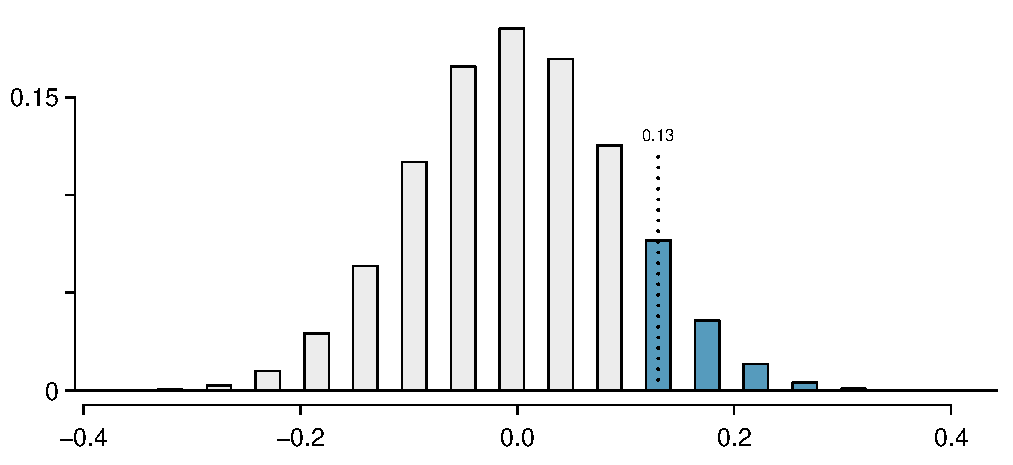
\includegraphics[width=0.8\textwidth]{02/figures/CPR_study/CPR_study_right_tail}
\caption{Null distribution of the point estimate, $\hat{p}_t - \hat{p}_c$. The shaded right tail shows observations that are at least as large as the observed difference,~0.13.}
\label{CPR_study_right_tail}
\end{figure}

The right tail area is about 0.13. (Note: it is only a coincidence that we also have $\hat{p}_t - \hat{p}_c=0.13$.) However, contrary to how we calculated the p-value in previous studies, the p-value of this test is not~0.13!

The p-value is defined as the chance we observe a result at least as favorable to the alternative hypothesis as the result (i.e.~the difference) we observe. In this case, any differences less than or equal to -0.13 would also provide equally strong evidence favoring the alternative hypothesis as a difference of 0.13, since -0.13 would correspond to 13\% higher survival rate in the control group than the treatment group. In Figure~\ref{CPR_study_p_value} we've also shaded these differences in the left tail of the distribution. These two shaded tails provide a visual representation of the p-value for a two-sided test.

%There is something different in this study than in the past studies: in this study, we are particularly interested in whether blood thinners increase \emph{or} decrease the risk of death in patients who undergo CPR before arriving at the hospital.\footnote{Realistically, we probably are interested in either direction in the past studies as well, and so we should have used the approach we now discuss in this section. However, for simplicity and the sake of not introducing too many concepts at once, we skipped over these details in earlier sections.} For example, there are chance differences of $\hat{p}_t - \hat{p}_c = -0.14$, that would have been stronger evidence against the null hypothesis as our observed difference of +0.13. Likewise, anything less than or equal -0.13 would provide as much evidence against the null hypothesis as +0.13, and for this reason, we must count both tails towards the p-value, as shown in Figure~\ref{CPR_study_p_value}.

\begin{figure}[ht]
\centering
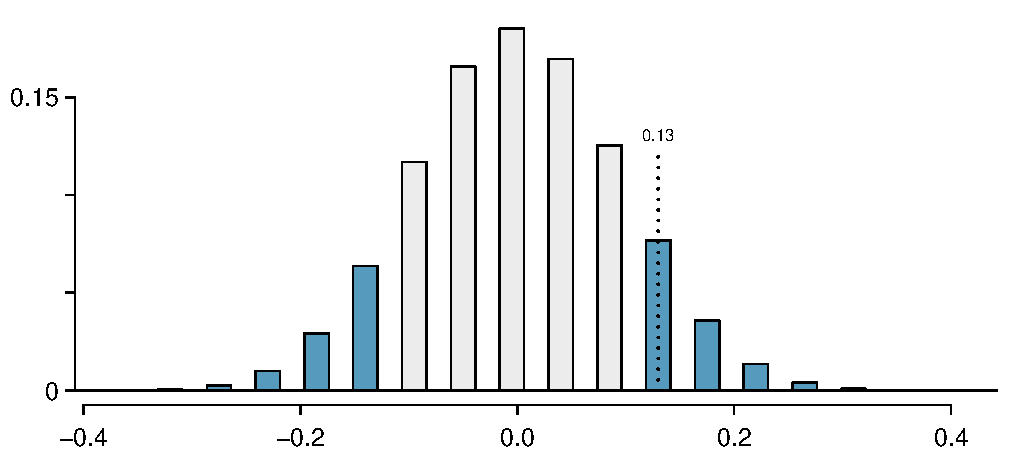
\includegraphics[width=0.8\textwidth]{02/figures/CPR_study/CPR_study_p_value}
\caption{Null distribution of the point estimate, $\hat{p}_t - \hat{p}_c$. All values that are at least as extreme as +0.13 but in either direction away from~0 are~shaded.}
\label{CPR_study_p_value}
\end{figure}

For a two-sided test, it is generally reasonable to take our single tail (in this case, 0.13) and double it to get the p-value: 0.26. Since this p-value is larger than 0.05, we do not reject the null hypothesis. That is, we do not find statistically significant evidence that the blood thinner has any influence on survival of patients who undergo CPR prior to arriving at the hospital. Once again, we can make a causal conclusion since this is an experiment.

\index{data!CPR and blood thinner|)}

\begin{termBox}{\tBoxTitle{Default to a two-sided test}
We want to be rigorous and keep an open mind when we analyze data and evidence. Use a one-sided hypothesis test only if you truly have interest in only one direction.}
\end{termBox}

\begin{termBox}{\tBoxTitle{Computing a p-value for a two-sided test}
First compute the p-value for one tail of the distribution, then double that value to get the two-sided p-value. That's it!}
\end{termBox}


\subsection{Controlling the Type~1 Error~rate}
\label{InflatingType1ErrorRate}

It is never okay to change two-sided tests to one-sided tests after observing the data. We explore the consequences of ignoring this advice in the next example.

\begin{example}{Using $\alpha=0.05$, we show that freely switching from two-sided tests to one-sided tests will lead us to make twice as many Type~1 Errors as intended.} \label{swappingHypAfterDataDoublesType1ErrorRate}
Suppose we are interested in finding any difference from 0. We've created a smooth-looking \term{null distribution} representing differences due to chance in Figure~\ref{type1ErrorDoublingExampleFigure}.

Suppose the sample difference was larger than 0. Then if we can flip to a one-sided test, we would use $H_A$: difference $> 0$. Now if we obtain any observation in the upper 5\% of the distribution, we would reject $H_0$ since the p-value would just be a the single tail. Thus, if the null hypothesis is true, we incorrectly reject the null hypothesis about 5\% of the time when the sample mean is above the null value, as shown in Figure~\ref{type1ErrorDoublingExampleFigure}.

Suppose the sample difference was smaller than 0. Then if we change to a one-sided test, we would use $H_A$: difference $< 0$. If the observed difference falls in the lower 5\% of the figure, we would reject $H_0$. That is, if the null hypothesis is true, then we would observe this situation about 5\% of the time.

By examining these two scenarios, we can determine that we will make a Type~1 Error $5\%+5\%=10\%$ of the time if we are allowed to swap to the ``best'' one-sided test for the data. This is twice the error rate we prescribed with our significance level: $\alpha=0.05$ (!).

\begin{figure}
\centering
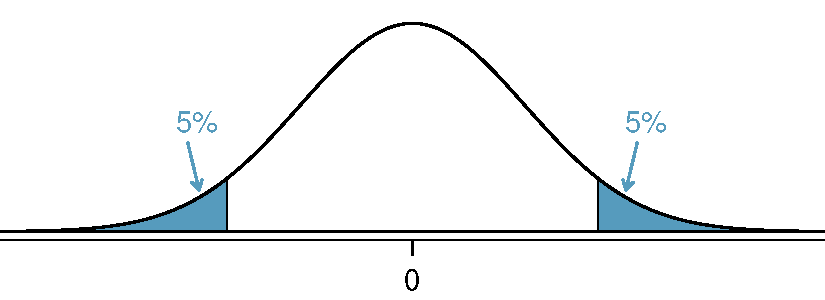
\includegraphics[width=0.7\textwidth]{02/figures/type1ErrorDoublingExampleFigure/type1ErrorDoublingExampleFigure}
\caption{The shaded regions represent areas where we would reject $H_0$ under the bad practices considered in Example~\ref{swappingHypAfterDataDoublesType1ErrorRate} when $\alpha = 0.05$.}
\label{type1ErrorDoublingExampleFigure}
\end{figure}

\end{example}

\begin{caution}{Hypothesis tests should be set up \emph{before} seeing the data}
{After observing data, it is tempting to turn a two-sided test into a one-sided test. Avoid this temptation. Hypotheses should be set up \emph{before} observing the data.}
\end{caution}

%\Comment{Should we scrap this subsection and example and just leave the caution box? Downside: weakens item 1 near the start of Section~\ref{IntroducingTwoSidedHypotheses}.}

\index{hypothesis testing!two tails|)}


\subsection{How to use a hypothesis test}

\noindent\textbf{Frame the research question in terms of hypotheses.} Hypothesis tests are appropriate for research questions that can be summarized into two competing hypotheses. The null hypothesis ($H_0$) usually represents a skeptical perspective or a perspective of no difference. The alternative hypothesis ($H_A$) usually represents a new view or a difference. \\

\noindent\textbf{Collect data with an observational study or experiment.} If a research question can be formed into two hypotheses, we can collect data to run a hypothesis test. If the research question focuses on associations between variables but does not concern causation, we would run an observational study. If the research question seeks a causal connection between two or more variables, then an experiment should be used. \\

\noindent\textbf{Analyze the data.} Choose an analysis technique appropriate for the data and identify the p-value. So far, we've only seen one analysis technique: randomization. Throughout the rest of this textbook, we'll encounter several new methods suitable for many other contexts. \\

\noindent\textbf{Form a conclusion.} Using the p-value from the analysis, determine whether the data provide statistically significant evidence against the null hypothesis. Also, be sure to write the conclusion in plain language so even non-statisticians understand the results.


%_________________
\section{Simulation case studies}
\label{SimulationCaseStudies}

Randomization is a statistical technique suitable for evaluating whether a difference in sample proportions is due to chance. In this section, we explore the situation where we focus on a single proportion, and we introduce a new simulation method.

\subsection{Medical consultant}

\index{data!medical consultant|(}
People providing an organ for donation sometimes seek the help of a special medical consultant. These consultants assist the patient in all aspects of the surgery, with the goal of reducing the possibility of complications during the medical procedure and recovery. Patients might choose a consultant based in part on the historical complication rate of the consultant's clients.

One consultant tried to attract patients by noting the average complication rate for liver donor surgeries in the US is about 10\%, but her clients have had only 3 complications in the 62 liver donor surgeries she has facilitated. She claims this is strong evidence that her work meaningfully contributes to reducing complications (and therefore she should be~hired!).

\begin{example}{We will let $p$ represent the true complication rate for liver donors working with this consultant. Estimate $p$ using the data, and label this value $\hat{p}$.}
The sample proportion for the complication rate is 3~complications divided by the 62~surgeries the consultant has worked on: $\hat{p} = 3/62 = 0.048$.
\end{example}

\begin{example}{Is it possible to assess the consultant's claim using the data?}
No. The claim is that there is a causal connection, but the data are observational. For example, maybe patients who can afford a medical consultant can afford better medical care, which can also lead to a lower complication rate.

While it is not possible to assess the causal claim, it is still possible to test for an association using these data. For this question we ask, could the low complication rate of $\hat{p} = 0.048$ be due to chance?
\end{example}

\begin{example}{We're going to conduct a hypothesis test for this setting. Should the test be one-sided or two-sided?}
The setting has been framed in the context of the consultant being helpful, but what if the consultant actually performed worse than the average? Would we care? More than ever! Since we care about a finding in either direction, we should run a two-sided~test.
\end{example}

\begin{exercise}\label{hypForAssessingConsultantWorkInLiverTransplants}
Write out hypotheses in both plain and statistical language to test for the association between the consultant's work and the true complication rate, $p$, for this consultant's clients.\footnote{$H_0$: There is no association between the consultant's contributions and the clients' complication rate. That~is, the complication rate for the consultant's clients is equal to the US average of 10\%. In statistical language, $p=0.10$. $H_A$: Patients who work with the consultant have a complication rate different than~10\%, i.e.~$p \neq 0.10$.}
\end{exercise}

\begin{termBox}{\tBoxTitle{Parameter for a hypothesis test}
A \term{parameter} for a hypothesis test is the ``true'' value of interest. We typically estimate the parameter using a point estimate from a sample of data.}
\end{termBox}

\begin{termBox}{\tBoxTitle{Null value of a hypothesis test}
The \term{null value} is the reference value for the parameter in $H_0$, and it is sometimes represented with the parameter's label with a~subscript 0, e.g.~$p_0$ (just like $H_0$).}
\end{termBox}

In this case study, the parameter is $p$ and the null value is $p_0 = 0.10$. We will use the p-value to quantify the possibility of a sample proportion ($\hat{p}$) this far from the null value. The p-value is computed based on the null distribution, which is the distribution of the test statistic if the null hypothesis were true. Just like we did using randomization for a difference in proportions, here we can simulate 62 new patients to see what result might happen if the complication rate was 0.10.

Each client can be simulated using a deck of cards. Take one red card, nine black cards, and mix them up. If the cards are well-shuffled, drawing the top card is one way of simulating the chance a patient has a complication if the true rate is 0.10: if the card is red, we say the patient had a complication, and if it is black then we say they did not have a complication. If we repeat this process 61 more times and compute the proportion of simulated patients with complications, $\hat{p}_{sim}$, then this sample proportion is exactly a sample from the null distribution.

\begin{exercise}
In a simulation of 62 patients, about how many would we expect to have had a complication?\footnote{About 10\% of the patients (6.2 on average) in the simulation will have a complication, though we will see a little variation from one simulation to the next.}
\end{exercise}

We conducted such a simulation. There were 5 simulated cases with a complication and 57 simulated cases without a complication: $\hat{p}_{sim} = 5/62 = 0.081$.

%\begin{example}{Is this one simulation enough to determine whether or not we should reject the null hypothesis from Exercise~\ref{hypForAssessingConsultantWorkInLiverTransplants}? Explain.}
%No. To assess the hypotheses, we need to see a distribution of many $\hat{p}_{sim}$, not just a single draw from this sampling distribution. We need to build a null distribution analogous to what we built using randomization.
%\end{example}

One simulation isn't enough to get a sense of the null distribution, so we repeated the simulation 10,000 times using a~computer. Figure~\ref{MedConsNullSim} shows the null distribution from these 10,000 simulations. The simulated proportions that are less than or equal to $\hat{p}=0.048$ are shaded. There were 1222 simulated sample proportions with $\hat{p}_{sim} \leq 0.048$, which represents a fraction 0.1222 of our simulations:
\begin{align*}
\text{left tail }
	= \frac{\text{Number of observed simulations with }\hat{p}_{sim}\leq\text{ 0.048}}{10000}
	= \frac{1222}{10000} = 0.1222
\end{align*}
However, this is not our p-value! Remember that we are conducting a two-sided test, so we should double the one-tail area to get the p-value:\footnote{This doubling approach is preferred even when the distribution isn't symmetric, as in this case.}
\begin{align*}
\text{p-value} = 2 \times \text{left tail} = 2 \times 0.1222 = 0.2444
\end{align*}

\begin{figure}[ht]
\centering
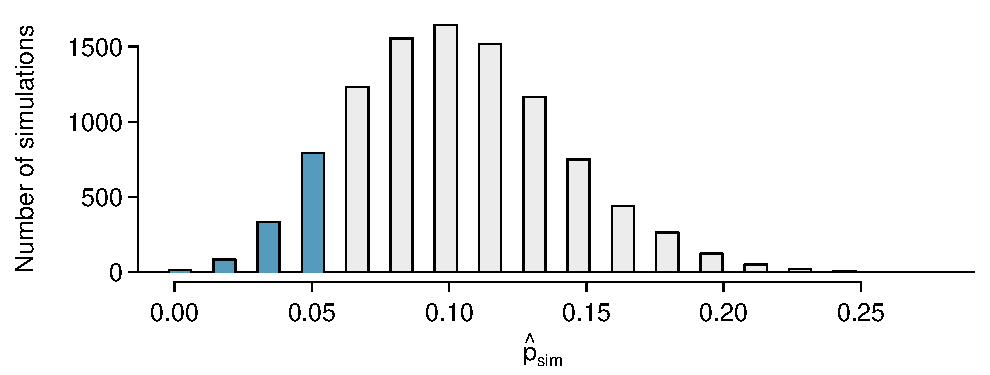
\includegraphics[width=0.9\textwidth]{02/figures/MedicalConsultant/MedConsNullSim}
\caption{The null distribution for $\hat{p}$, created from 10,000 simulated studies. The left tail contains 12.22\% of the simulations. We double this value to get the p-value.}
\label{MedConsNullSim}
\end{figure}

\begin{exercise} \label{plainLanguageExplanationOfHTConclusionForLiverDonorSurgicalConsultant}
Because the p-value is 0.2444, which is larger than the significance level 0.05, we do not reject the null hypothesis. Explain what this means in plain language in the context of the problem.\footnote{The data do not provide strong evidence that the consultant's work is associated with a lower (or higher) rate of surgery complications than the general rate of 10\%.}
\end{exercise}

\begin{example}{Does the conclusion in Exercise~\ref{plainLanguageExplanationOfHTConclusionForLiverDonorSurgicalConsultant} imply there is no real association between the surgical consultant's work and the risk of complications? Explain.}
No. It might be that the consultant's work is associated with a lower or higher risk of complications. However, the data did not provide enough information to reject the null hypothesis. %However, we currently don't have enough data to say whether the corresponding complication rate is any different than 0.10.
\index{data!medical consultant|)}
\end{example}


%_________________
\subsection{Tappers and listeners}

Here's a game you can try with your friends or family: pick a simple, well-known song, tap that tune on your desk, and see if the other person can guess the song. In this simple game, you are the tapper, and the other person is the listener.

A Stanford University graduate student named Elizabeth Newton conducted an experiment using the tapper-listener game.\footnote{This case study is described in \emph{\href{http://www.openintro.org/redirect.php?go=made-to-stick&redirect=textbook_pdf_preliminary}{Made to Stick}} by Chip and Dan Heath. Little known fact: the teaching principles behind many OpenIntro resources are based on Made to Stick.} In her study, she recruited 120 tappers and 120 listeners into the study. About 50\% of the tappers expected that the listener would be able to guess the song. Newton wondered, is 50\% a reasonable expectation?

Newton's research question can be framed into two hypotheses:
\begin{itemize}
\setlength{\itemsep}{0mm}
\item[$H_0$:] The tappers are correct, and generally 50\% of the time listeners are able to guess the tune. $p = 0.50$
\item[$H_A$:] The tappers are incorrect, and either more than or less than 50\% of listeners will be able to guess the tune. $p \neq 0.50$
\end{itemize}

In Newton's study, only 3 out of 120 listeners ($\hat{p} = 0.025$) were able to guess the tune! From the perspective of the null hypothesis, we might wonder, how likely is it that we would get this result from chance alone? That is, what's the chance we would happen to see such a small fraction if $H_0$ were true and the true correct-guess rate is 0.50?

We will again use a simulation. To simulate 120 games under the null hypothesis ($p = 0.50$), we could flip a coin 120 times. Each time the coin came up heads, this could represent the listener guessing correctly, and tails would represent the listener guessing incorrectly. For example, we can simulate 5 tapper-listener pairs by flipping a coin five times:
\begin{center}
\begin{tabular}{ccc ccc ccc c}
H & H & T & H & T \\
Correct & Correct & Wrong & Correct & Wrong \\
\end{tabular}
\end{center}
After flipping the coin 120 times, we got 56 heads for $\hat{p}_{sim} = 0.467$. As we did with the randomization technique, seeing what would happen with one simulation isn't enough. In order to evaluate whether our originally observed proportion of 0.025 is unusual or not, we should generate more simulations. Here we've repeated this simulation eight times:
\begin{align*}
0.558 \quad 0.517 \quad 0.467 \quad 0.458 \quad
0.525 \quad 0.425 \quad 0.458 \quad 0.492
\end{align*} % round(rbinom(8, 120, 0.5) / 120, 3)
As before, we'll run a total of 10,000 simulations using a computer. Figure~\ref{TappersAndListenersNullDistribution} shows the results of these simulations. Even in these 10,000 simulations, we don't see any results close to 0.025.

\begin{figure}[ht]
\centering
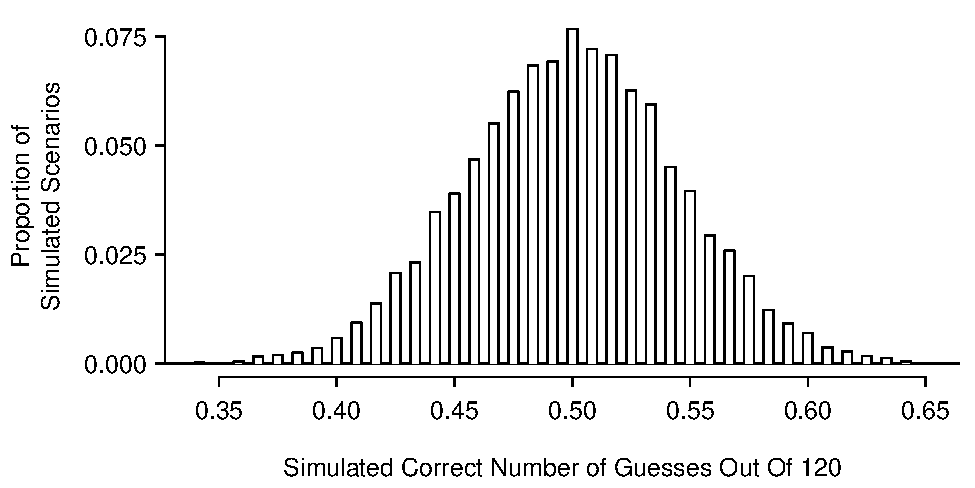
\includegraphics[width=0.8\textwidth]{02/figures/TappersAndListeners/TappersAndListenersNullDistribution}
\caption{Results from 10,000 simulations of the tapper-listener study where guesses are correct half of the time.}
\label{TappersAndListenersNullDistribution}
\end{figure}

\begin{exercise}
What is the p-value for the hypothesis test?\footnote{The p-value is the chance of seeing the data summary or something more in favor of the alternative hypothesis. Since we didn't observe anything even close to just 3 correct, the p-value will be small, around 1-in-10,000 or smaller.}
\end{exercise}

\begin{exercise}
Do the data provide statistically significant evidence against the null hypothesis? State an appropriate conclusion in the context of the research question.\footnote{The p-value is less than 0.05, so we reject the null hypothesis. There is statistically significant evidence, and the data provide strong evidence that the chance a listener will guess the correct tune is less than 50\%.}
\end{exercise}


%_________________
\section{Central Limit Theorem}
\label{CLTsection}

We've encountered four case studies so far this chapter. While they differ in the settings, in their outcomes, and also in the technique we've used to analyze the data, they all have something in common: the general shape of the null distribution.

\subsection{Sampling distribution from the case studies}

Figure~\ref{FourCaseStudies} shows the null distributions in each of the four case studies where we ran 10,000 simulations.

\begin{figure}[ht]
\centering
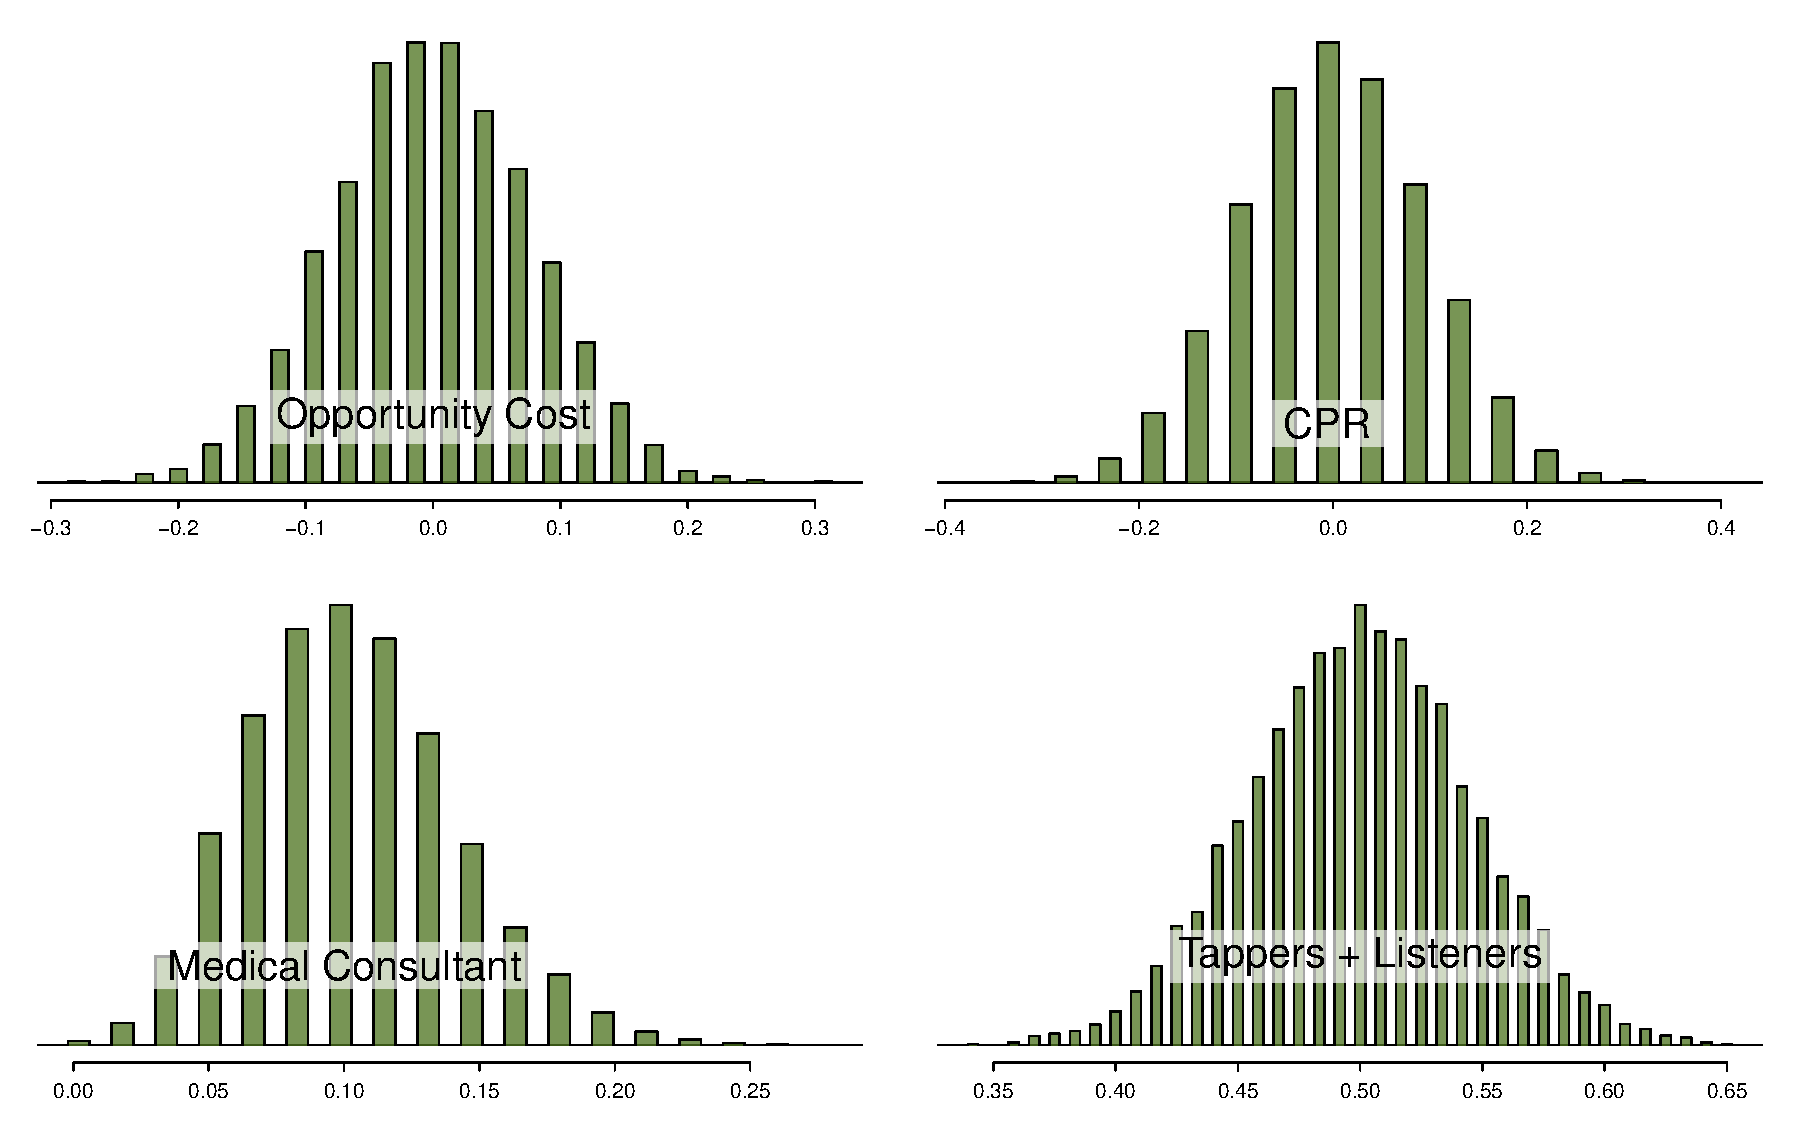
\includegraphics[width=0.97\textwidth]{02/figures/FourCaseStudies/FourCaseStudies}
\caption{The null distribution for each of the four case studies presented in Sections~\ref{caseStudyOpportunityCost}-\ref{SimulationCaseStudies}.}
\label{FourCaseStudies}
\end{figure}

\begin{exercise}
Describe the shape of the distributions and note anything that you find interesting.\footnote{In general, the distributions are reasonably symmetric. The case study for the medical consultant is the only distribution with any evident skew.}
\end{exercise}

As we observed in Chapter~\ref{introductionToData}, it's common for distributions to be skewed or contain outliers. However, the null distributions we've so far encountered have all looked somewhat similar and, for the most part, symmetric. They all resemble a bell-shaped curve. This is not a coincidence, but rather, is guaranteed by  mathematical theory.

\begin{termBox}{\tBoxTitle{Central Limit Theorem for proportions}
If we look at a proportion (or difference in proportions) and the scenario satisfies certain conditions, then the sample proportion (or difference in proportions) will appear to follow a bell-shaped curve called the \emph{normal distribution}.\index{Central Limit Theorem}\index{Central Limit Theorem!proportion}\index{Central Limit Theorem!difference in proportions}}
\end{termBox}

An example of a perfect normal distribution is shown in Figure~\ref{simpleNormal}. Imagine laying a normal curve over each of the four null distributions in Figure~\ref{FourCaseStudies}. While the mean and standard deviation may change for each plot, the general shape remains roughly intact.

\begin{figure}[ht]
\centering
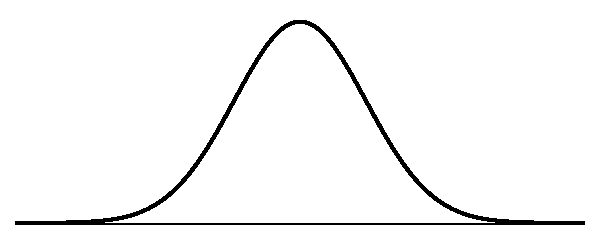
\includegraphics[width=0.5\textwidth]{02/figures/simpleNormal/simpleNormal}
\caption{A normal curve.}
\label{simpleNormal}
\end{figure}

Mathematical theory guarantees that a sample proportion or a difference in sample proportions will follow something that resembles a normal distribution when certain conditions are met. These conditions fall into two categories:
\begin{description}
\item[Oservations in the sample are independent.] Independence is guaranteed when we take a random sample from a population. It can also be guaranteed if we randomly divide individuals into treatment and control groups.
\item[The sample is large enough.] The sample size cannot be too small. What qualifies as small differs from one context to the next, and we'll provide suitable guidelines for proportions in Chapter~\ref{inferenceForCategoricalData}.
\end{description}

So far we've had no need to use the normal distribution. We've been able to answer our questions somewhat easily using simulation techniques. However, soon this will change. Simulating data can be non-trivial. For example, some scenarios that we will encounter in Chapters~\ref{linRegrForTwoVar} and~\ref{multipleAndLogisticRegression} would require extremely complex simulations. Instead, the normal distribution -- and other distributions like it -- offer us a general framework that applies to a very large number of settings.


\subsection{Examples of future settings we will consider}

Below we introduce three new settings where the normal distribution will be useful but constructing suitable simulations may be difficult.

\begin{example}{The opportunity cost study determined that students are thriftier if they are reminded that saving money now means they can spend the money later. The study's point estimate for the estimated impact was 20\%, meaning 20\% fewer students would move forward with a DVD purchase in the study scenario. However, as we've learned, point estimates aren't perfect -- they only provide an approximation of the truth.}
It would be useful if we could provide a \emph{range of plausible values} for the impact, more formally known as a \term{confidence interval}. It is often difficult to construct a reliable confidence interval in many situations using simulations.\footnote{The percentile bootstrap method has been put forward as an alternative. However, simulations show that this method is consistently less robust than than the normal distribution. For more information, visit \href{http://openintro.org/bootstrap}{openintro.org/bootstrap}.} However, doing so is reasonably straightforward using the normal distribution. We'll tackle this topic in Section~\ref{ConfidenceIntervals}.
\end{example}

\begin{example}{Book prices were collected for 73 courses at UCLA in Spring 2010. Data were collected from both the UCLA Bookstore and Amazon. The differences in these prices are shown in Figure~\ref{diffInTextbookPricesS10_CLTsection}. The mean difference in the price of the books was \$12.76, and we might wonder, does this provide strong evidence that the prices differ between the two book sellers?}
Here again we can apply the normal distribution, this time in the context of numerical data. We'll explore this example and construct such a confidence interval in Section~\ref{pairedData}.
\end{example}

\begin{figure}[ht]
\centering
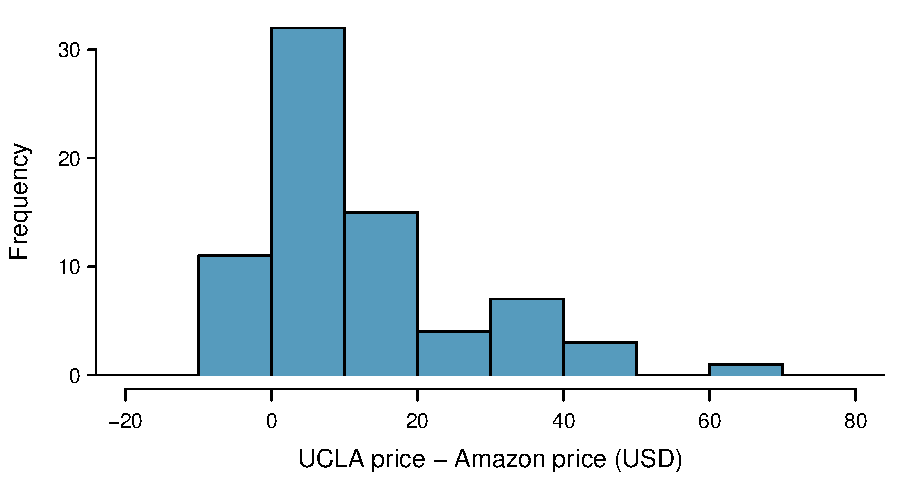
\includegraphics[width=0.7\textwidth]{05/figures/textbooksS10/diffInTextbookPricesS10}
\caption{Histogram of the difference in price for each book sampled. These data are strongly skewed.\index{skew!example: strong}}
\label{diffInTextbookPricesS10_CLTsection}
\end{figure}

\begin{example}{Elmhurst College in Illinois released anonymized data for family income and financial support provided by the school for Elmhurst's first-year students in 2011. Figure~\ref{elmhurstScatterWLSROnly_CLTsection} shows a \emph{regression line} fit to a scatterplot of a sample of the data. One question we will ask is, do the data show a real trend, or is the trend we observe reasonably explained by chance?}
In Chapter~\ref{linRegrForTwoVar} we'll learn how to apply least squares regression to quantify the trend and quantify whether or not that trend can be explained by chance alone. For this case study, we can again use the normal distribution to help us answer this question.
\end{example}

\begin{figure}[ht]
\centering
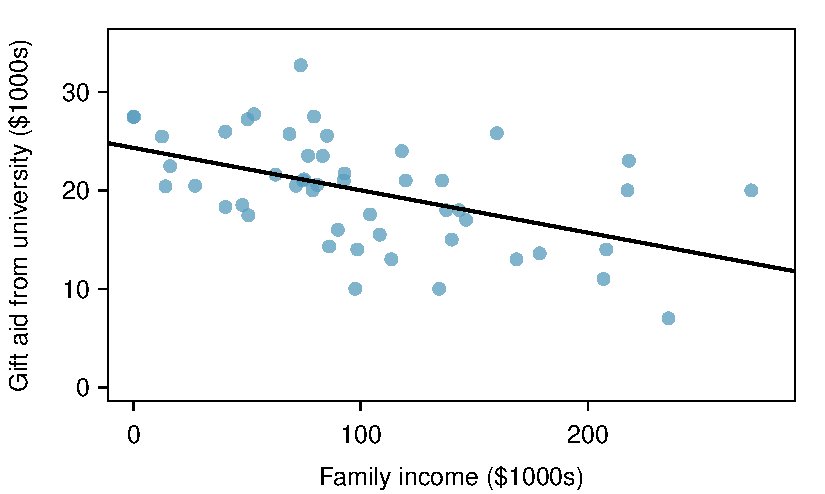
\includegraphics[width=0.7\textwidth]{07/figures/elmhurstPlots/elmhurstScatterWLSROnly}
\caption{Gift aid and family income for a random sample of 50 first-year students from Elmhurst College, shown with a regression line.}
\label{elmhurstScatterWLSROnly_CLTsection}
\end{figure}

These examples highlight the value of the normal distribution approach. However, before we can get started with applying the normal distribution to statistical inference, it is necessary to become familiar with the mechanics of the normal distribution. In Section~\ref{normalDist} we discuss characteristics of the normal distribution, explore examples of data that follow a normal distribution, and learn a new plotting technique that is useful for evaluating whether a data set roughly follows the normal distribution. In Sections~\ref{ApplyingTheNormalModel} and~\ref{ConfidenceIntervals}, we apply this new knowledge in the context of hypothesis tests and confidence intervals.


%_________________
\section{Normal distribution}
\label{normalDist}

\index{normal distribution|(}

Among all the distributions we see in statistics, one is overwhelmingly the most common. The symmetric, unimodal, bell curve is ubiquitous throughout statistics. It is so common that people often know it as the \term{normal curve}, \term{normal model}, or \termsub{normal distribution}{distribution!normal}.\footnote{It is also introduced as the Gaussian distribution after Frederic Gauss, the first person to formalize its mathematical expression.} Under certain conditions, sample proportions, sample means, and differences can be modeled using the normal distribution. Additionally, some variables such as SAT scores and heights of US adult males closely follow the normal distribution.

\begin{termBox}{\tBoxTitle{Normal distribution facts}
Many summary statistics and variables are nearly normal, but none are exactly normal. Thus the normal distribution, while not perfect for any single problem, is very useful for a variety of problems. We will use it in data exploration and to solve important problems in statistics.\vspace{0.7mm}}
\end{termBox}

In this section, we will discuss the normal distribution in the context of data to (1) become familiar with normal distribution techniques and (2) learn how to evaluate whether data are nearly normal. In Sections~\ref{ApplyingTheNormalModel}-\ref{ConfidenceIntervals} and beyond, we'll move our discussion to focus on applying the normal distribution and other related distributions to model point estimates for hypothesis tests and for constructing confidence intervals.

\subsection{Normal distribution model}
\label{NormalDistributionModelSubsection}

The normal distribution always describes a symmetric, unimodal, bell-shaped curve. However, these curves can look different depending on the details of the model. Specifically, the normal model can be adjusted using two parameters: mean and standard deviation. As you can probably guess, changing the mean shifts the bell curve to the left or right, while changing the standard deviation stretches or constricts the curve. Figure~\ref{twoSampleNormals} shows the normal distribution with mean $0$ and standard deviation $1$ in the left panel and the normal distributions with mean $19$ and standard deviation $4$ in the right panel. Figure~\ref{twoSampleNormalsStacked} shows these distributions on the same axis.

\begin{figure}[hht]
\centering
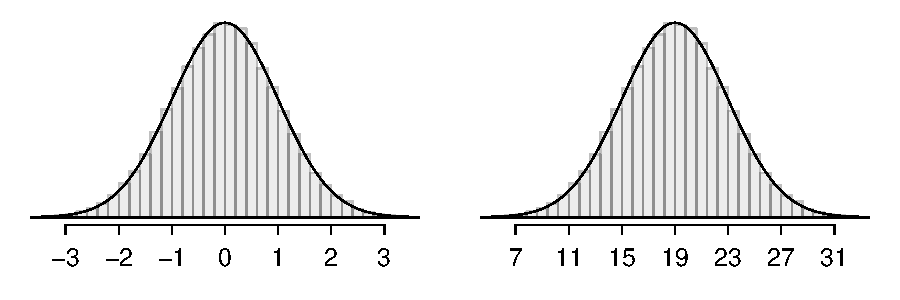
\includegraphics[width=0.9\textwidth]{02/figures/twoSampleNormals/twoSampleNormals}
\caption{Both curves represent the normal distribution, however, they differ in their center and spread. The normal distribution with mean 0 and standard deviation 1 is called the \term{standard normal distribution}.}
\label{twoSampleNormals}
\end{figure}

\begin{figure}[hht]
\centering
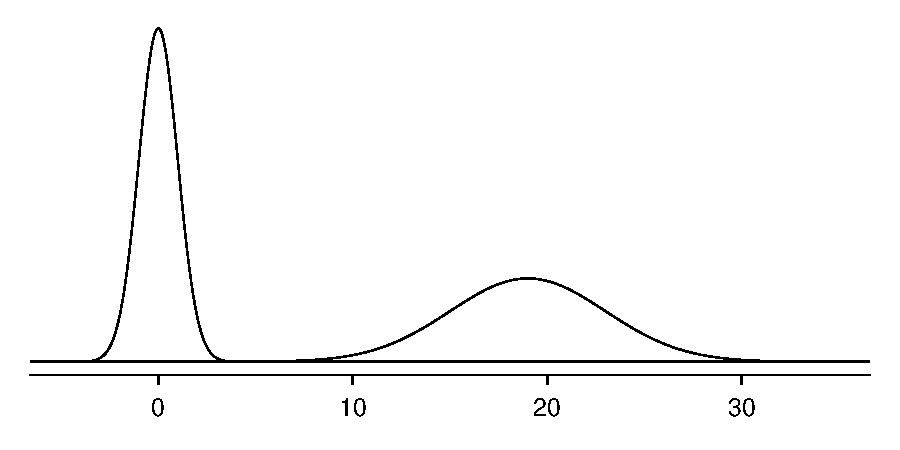
\includegraphics[width=0.62\textwidth]{02/figures/twoSampleNormalsStacked/twoSampleNormalsStacked}
\caption{The normal models shown in Figure~\ref{twoSampleNormals} but plotted together and on the same scale.}
\label{twoSampleNormalsStacked}
\end{figure}

If a normal distribution has mean $\mu$ and standard deviation $\sigma$, we may write the distribution as $N(\mu, \sigma)$\marginpar[\raggedright\vspace{-5mm}

$N(\mu, \sigma)$\vspace{1mm}\\\footnotesize Normal dist.\\with mean $\mu$\\\& st. dev. $\sigma$]{\raggedright\vspace{-5mm}

$N(\mu, \sigma)$\vspace{1mm}\\\footnotesize Normal dist.\\with mean $\mu$\\\& st. dev. $\sigma$}. The two distributions in Figure~\ref{twoSampleNormalsStacked} can be written as
\begin{align*}
N(\mu=0,\sigma=1)\quad\text{and}\quad N(\mu=19,\sigma=4)
\end{align*}
Because the mean and standard deviation describe a normal distribution exactly, they are called the distribution's \termsub{parameters}{parameter}.

\begin{exercise}
Write down the short-hand for a normal distribution with (a)~mean~5 and standard deviation~3, (b)~mean~-100 and standard deviation~10, and (c)~mean~2 and standard deviation~9.\footnote{(a)~$N(\mu=5,\sigma=3)$. (b)~$N(\mu=-100, \sigma=10)$. (c)~$N(\mu=2, \sigma=9)$.}
\end{exercise}

\subsection{Standardizing with Z scores}

\begin{example}{Table~\ref{satACTstats} shows the mean and standard deviation for total scores on the SAT and ACT. The distribution of SAT and ACT scores are both nearly normal. Suppose Ann scored 1800 on her SAT and Tom scored 24 on his ACT. Who performed better?}\label{actSAT}
We use the standard deviation as a guide. Ann is 1 standard deviation above average on the SAT: $1500 + 300=1800$. Tom is 0.6 standard deviations above the mean on the ACT: $21+0.6\times 5=24$. In Figure~\ref{satActNormals}, we can see that Ann tends to do better with respect to everyone else than Tom did, so her score was better.
\end{example}

\begin{table}[ht]
\centering
\begin{tabular}{l r r}
  \hline
  & SAT & ACT \\
  \hline
Mean \hspace{0.3cm} & 1500 & 21 \\
SD & 300 & 5 \\
   \hline
\end{tabular}
\caption{Mean and standard deviation for the SAT and ACT.}
\label{satACTstats}
\end{table}

\begin{figure}[ht]
\centering
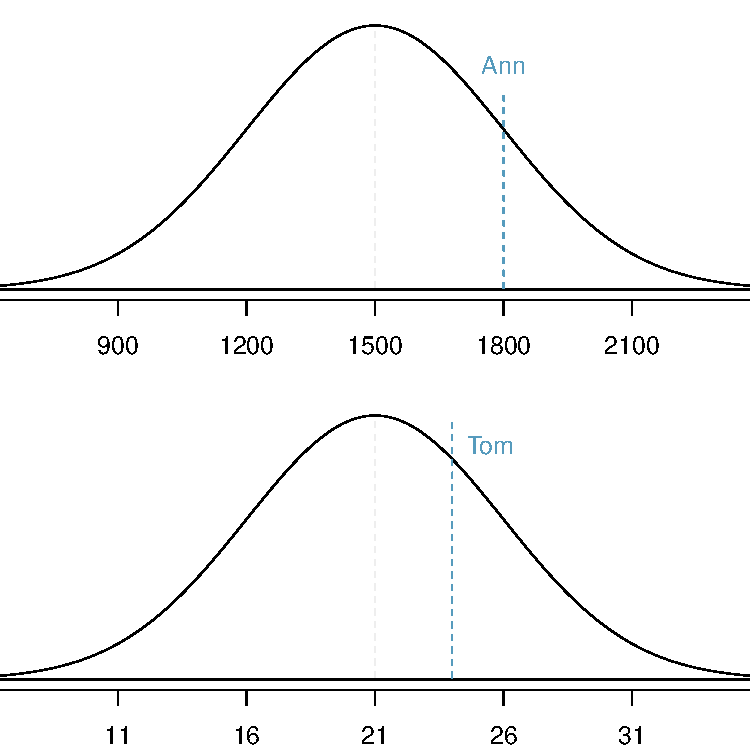
\includegraphics[width=65mm]{02/figures/satActNormals/satActNormals}
\caption{Ann's and Tom's scores shown with the distributions of SAT and ACT scores.}
\label{satActNormals}
\end{figure}

Example~\ref{actSAT} used a standardization technique called a Z score, a method most commonly employed for nearly normal observations but that may be used with any distribution. The \term{Z score}\marginpar[\raggedright\vspace{-3mm}

$Z$\vspace{1mm}\\\footnotesize Z score, the\\standardized\\observation]{\raggedright\vspace{-3mm}

$Z$\vspace{1mm}\\\footnotesize Z score, the\\standardized\\observation}\index{Z@$Z$} of an observation is defined as the number of standard deviations it falls above or below the mean. If the observation is one standard deviation above the mean, its Z score is 1. If it is 1.5 standard deviations \emph{below} the mean, then its Z score is -1.5. If $x$ is an observation from a distribution $N(\mu, \sigma)$, we define the Z score mathematically as
\begin{eqnarray*}
Z = \frac{x-\mu}{\sigma}
\end{eqnarray*}
Using $\mu_{SAT}=1500$, $\sigma_{SAT}=300$, and $x_{Ann}=1800$, we find Ann's Z score:
\begin{eqnarray*}
Z_{Ann} = \frac{x_{Ann} - \mu_{SAT}}{\sigma_{SAT}} = \frac{1800-1500}{300} = 1
\end{eqnarray*}

\begin{termBox}{\tBoxTitle{The Z score}
The Z score of an observation is the number of standard deviations it falls above or below the mean. We compute the Z score for an observation $x$ that follows a distribution with mean $\mu$ and standard deviation $\sigma$ using
\begin{eqnarray*}
Z = \frac{x-\mu}{\sigma}
\end{eqnarray*}}
\end{termBox}

\begin{exercise}
Use Tom's ACT score, 24, along with the ACT mean and standard deviation to compute his Z score.\footnote{$Z_{Tom} = \frac{x_{Tom} - \mu_{ACT}}{\sigma_{ACT}} = \frac{24 - 21}{5} = 0.6$}
\end{exercise}

Observations above the mean always have positive Z scores while those below the mean have negative Z scores. If an observation is equal to the mean (e.g. SAT score of 1500), then the Z score is $0$.

\begin{exercise}
Let $X$ represent a random variable from $N(\mu=3, \sigma=2)$, and suppose we observe $x=5.19$. (a) Find the Z score of $x$. (b) Use the Z score to determine how many standard deviations above or below the mean $x$ falls.\footnote{(a) Its Z score is given by $Z = \frac{x-\mu}{\sigma} = \frac{5.19 - 3}{2} = 2.19/2 = 1.095$. (b) The observation $x$ is 1.095 standard deviations \emph{above} the mean. We know it must be above the mean since $Z$ is positive.}
\end{exercise}

\begin{exercise} \label{headLZScore}
Head lengths of brushtail possums follow a nearly normal distribution with mean 92.6 mm and standard deviation 3.6 mm. Compute the Z scores for possums with head lengths of 95.4 mm and 85.8 mm.\footnote{For $x_1=95.4$ mm: $Z_1 = \frac{x_1 - \mu}{\sigma} = \frac{95.4 - 92.6}{3.6} = 0.78$. For $x_2=85.8$ mm: $Z_2 = \frac{85.8 - 92.6}{3.6} = -1.89$.}
\end{exercise}

We can use Z scores to roughly identify which observations are more unusual than others. One observation $x_1$ is said to be more unusual than another observation $x_2$ if the absolute value of its Z score is larger than the absolute value of the other observation's Z score: $|Z_1| > |Z_2|$. This technique is especially insightful when a distribution is symmetric.

\begin{exercise}
Which of the observations in Exercise~\ref{headLZScore} is more unusual?\footnote{Because the \emph{absolute value} of Z score for the second observation is larger than that of the first, the second observation has a more unusual head length.}
\end{exercise}


\subsection{Normal probability table}

\begin{example}{Ann from Example~\ref{actSAT} earned a score of 1800 on her SAT with a corresponding $Z=1$. She would like to know what percentile she falls in among all SAT test-takers.}
Ann's \term{percentile} is the percentage of people who earned a lower SAT score than Ann. We shade the area representing those individuals in Figure~\ref{satBelow1800}. The total area under the normal curve is always equal to 1, and the proportion of people who scored below Ann on the SAT is equal to the \emph{area} shaded in Figure~\ref{satBelow1800}: 0.8413. In other words, Ann is in the $84^{th}$ percentile of SAT takers.
\end{example}

\begin{figure}[htb]
   \centering
   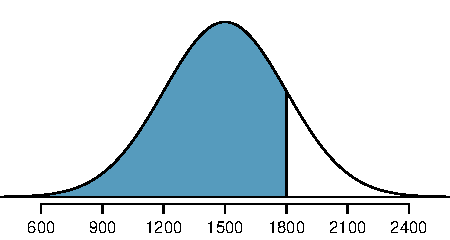
\includegraphics[height=1.5in]{02/figures/satBelow1800/satBelow1800}
   \caption{The normal model for SAT scores, shading the area of those individuals who scored below Ann.}
   \label{satBelow1800}
\end{figure}

We can use the normal model to find percentiles. A \term{normal probability table}, which lists Z scores and corresponding percentiles, can be used to identify a percentile based on the Z score (and vice versa). Statistical software can also be used.

A normal probability table is given in Appendix~\vref{normalProbabilityTable} and abbreviated in Table~\ref{zTableShort}. We use this table to identify the percentile corresponding to any particular Z score. For instance, the percentile of $Z=0.43$ is shown in row $0.4$ and column $0.03$ in Table~\ref{zTableShort}: 0.6664, or the $66.64^{th}$ percentile. Generally, we round $Z$ to two decimals, identify the proper row in the normal probability table up through the first decimal, and then determine the column representing the second decimal value. The intersection of this row and column is the percentile of the observation.

\begin{figure}
\centering
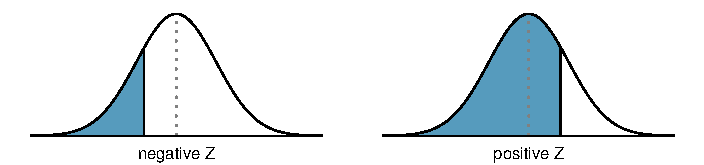
\includegraphics[width=0.8\textwidth]{02/figures/normalTails/normalTails}
\caption{The area to the left of $Z$ represents the percentile of the observation.}
\label{normalTails}
\end{figure}

\begin{table}
\centering
\begin{tabular}{c | rrrrr | rrrrr |}
  \cline{2-11}
&&&& \multicolumn{4}{c}{Second decimal place of $Z$} &&& \\
  \cline{2-11}
$Z$ & 0.00 & 0.01 & 0.02 & \highlightT{0.03} & \highlightO{0.04} & 0.05 & 0.06 & 0.07 & 0.08 & 0.09 \\
  \hline
  \hline
0.0 & \scriptsize{0.5000} & \scriptsize{0.5040} & \scriptsize{0.5080} & \scriptsize{0.5120} & \scriptsize{0.5160} & \scriptsize{0.5199} & \scriptsize{0.5239} & \scriptsize{0.5279} & \scriptsize{0.5319} & \scriptsize{0.5359} \\
  0.1 & \scriptsize{0.5398} & \scriptsize{0.5438} & \scriptsize{0.5478} & \scriptsize{0.5517} & \scriptsize{0.5557} & \scriptsize{0.5596} & \scriptsize{0.5636} & \scriptsize{0.5675} & \scriptsize{0.5714} & \scriptsize{0.5753} \\
  0.2 & \scriptsize{0.5793} & \scriptsize{0.5832} & \scriptsize{0.5871} & \scriptsize{0.5910} & \scriptsize{0.5948} & \scriptsize{0.5987} & \scriptsize{0.6026} & \scriptsize{0.6064} & \scriptsize{0.6103} & \scriptsize{0.6141} \\
%  May comment out 0.0-0.2 to make extra space. Then insert the following line:
%  $\vdots$ &   $\vdots$ &   $\vdots$ &   $\vdots$ &   $\vdots$ &   $\vdots$ &   $\vdots$ &   $\vdots$ &   $\vdots$ &   $\vdots$ &   $\vdots$ \\
  0.3 & \scriptsize{0.6179} & \scriptsize{0.6217} & \scriptsize{0.6255} & \scriptsize{0.6293} & \scriptsize{0.6331} & \scriptsize{0.6368} & \scriptsize{0.6406} & \scriptsize{0.6443} & \scriptsize{0.6480} & \scriptsize{0.6517} \\
\highlightT{0.4} & \scriptsize{0.6554} & \scriptsize{0.6591} & \scriptsize{0.6628} & \highlightT{\scriptsize{0.6664}} & \scriptsize{0.6700} & \scriptsize{0.6736} & \scriptsize{0.6772} & \scriptsize{0.6808} & \scriptsize{0.6844} & \scriptsize{0.6879} \\
  \hline
  0.5 & \scriptsize{0.6915} & \scriptsize{0.6950} & \scriptsize{0.6985} & \scriptsize{0.7019} & \scriptsize{0.7054} & \scriptsize{0.7088} & \scriptsize{0.7123} & \scriptsize{0.7157} & \scriptsize{0.7190} & \scriptsize{0.7224} \\
  0.6 & \scriptsize{0.7257} & \scriptsize{0.7291} & \scriptsize{0.7324} & \scriptsize{0.7357} & \scriptsize{0.7389} & \scriptsize{0.7422} & \scriptsize{0.7454} & \scriptsize{0.7486} & \scriptsize{0.7517} & \scriptsize{0.7549} \\
  0.7 & \scriptsize{0.7580} & \scriptsize{0.7611} & \scriptsize{0.7642} & \scriptsize{0.7673} & \scriptsize{0.7704} & \scriptsize{0.7734} & \scriptsize{0.7764} & \scriptsize{0.7794} & \scriptsize{0.7823} & \scriptsize{0.7852} \\
\highlightO{0.8} & \scriptsize{0.7881} & \scriptsize{0.7910} & \scriptsize{0.7939} & \scriptsize{0.7967} & \highlightO{\scriptsize{0.7995}} & \scriptsize{0.8023} & \scriptsize{0.8051} & \scriptsize{0.8078} & \scriptsize{0.8106} & \scriptsize{0.8133} \\
  0.9 & \scriptsize{0.8159} & \scriptsize{0.8186} & \scriptsize{0.8212} & \scriptsize{0.8238} & \scriptsize{0.8264} & \scriptsize{0.8289} & \scriptsize{0.8315} & \scriptsize{0.8340} & \scriptsize{0.8365} & \scriptsize{0.8389} \\
  \hline
  \hline
  1.0 & \scriptsize{0.8413} & \scriptsize{0.8438} & \scriptsize{0.8461} & \scriptsize{0.8485} & \scriptsize{0.8508} & \scriptsize{0.8531} & \scriptsize{0.8554} & \scriptsize{0.8577} & \scriptsize{0.8599} & \scriptsize{0.8621} \\
  1.1 & \scriptsize{0.8643} & \scriptsize{0.8665} & \scriptsize{0.8686} & \scriptsize{0.8708} & \scriptsize{0.8729} & \scriptsize{0.8749} & \scriptsize{0.8770} & \scriptsize{0.8790} & \scriptsize{0.8810} & \scriptsize{0.8830} \\
  $\vdots$ &   $\vdots$ &   $\vdots$ &   $\vdots$ &   $\vdots$ &   $\vdots$ &   $\vdots$ &   $\vdots$ &   $\vdots$ &   $\vdots$ &   $\vdots$ \\
   \hline
\end{tabular}
\caption{A section of the normal probability table. The percentile for a normal random variable with $Z=0.43$ has been \highlightT{highlighted}, and the percentile closest to 0.8000 has also been \highlightO{highlighted}.}
\label{zTableShort}
\end{table}

We can also find the Z score associated with a percentile. For example, to identify Z for the $80^{th}$ percentile, we look for the value closest to 0.8000 in the middle portion of the table: 0.7995. We determine the Z score for the $80^{th}$ percentile by combining the row and column Z values: 0.84.

\begin{exercise}
Determine the proportion of SAT test takers who scored better than Ann on the SAT.\footnote{If 84\% had lower scores than Ann, the number of people who had better scores must be 16\%. (Generally ties are ignored when the normal model, or any other continuous distribution, is used.)}
\end{exercise}


\subsection{Normal probability examples}

Cumulative SAT scores are approximated well by a normal model, $N(\mu=1500, \sigma=300)$.

\begin{example}{Shannon is a randomly selected SAT taker, and nothing is known about Shannon's SAT aptitude. What is the probability Shannon scores at least 1630 on her SATs?}\label{satAbove1630Exam}
First, always draw and label a picture of the normal distribution. (Drawings need not be exact to be useful.) We are interested in the chance she scores above 1630, so we shade this upper tail:
\begin{center}
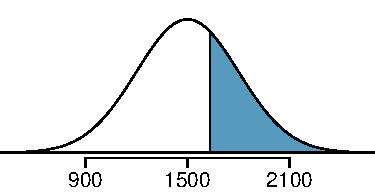
\includegraphics[height=0.9in]{02/figures/satAbove1630/satAbove1630}
\end{center}
The picture shows the mean and the values at 2 standard deviations above and below the mean. The simplest way to find the shaded area under the curve makes use of the Z score of the cutoff value. With $\mu=1500$, $\sigma=300$, and the cutoff value $x=1630$, the Z score is computed as
\begin{eqnarray*}
Z = \frac{x - \mu}{\sigma} = \frac{1630 - 1500}{300} = \frac{130}{300} = 0.43
\end{eqnarray*}
We look up the percentile of $Z=0.43$ in the normal probability table shown in Table~\ref{zTableShort} or in Appendix~\vref{normalProbabilityTable}, which yields 0.6664. However, the percentile describes those who had a Z score \emph{lower} than 0.43. To find the area \emph{above} $Z=0.43$, we compute one minus the area of the lower tail:
\begin{center}
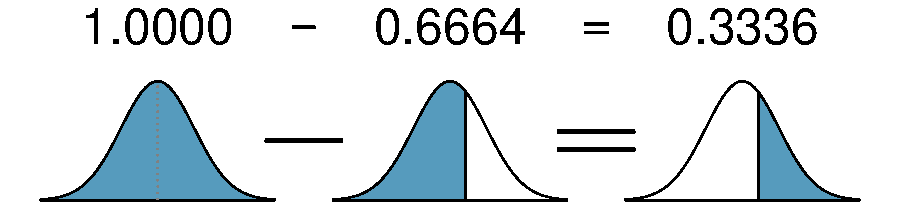
\includegraphics[height=0.8in]{02/figures/subtractingArea/subtractingArea}
\end{center}
The probability Shannon scores at least 1630 on the SAT is 0.3336.
\end{example}

\begin{tipBox}{\tipBoxTitle{always draw a picture first, and find the Z score second}
For any normal probability situation, \emph{always always always} draw and label the normal curve and shade the area of interest first. The picture will provide an estimate of the probability. \vspace{3mm}

After drawing a figure to represent the situation, identify the Z score for the observation of interest.\vspace{1mm}}
\end{tipBox}

\begin{exercise}
If the probability of Shannon scoring at least 1630 is 0.3336, then what is the probability she scores less than 1630? Draw the normal curve representing this exercise, shading the lower region instead of the upper one.\footnote{We found the probability in Example~\ref{satAbove1630Exam}: 0.6664. A picture for this exercise is represented by the shaded area below ``0.6664'' in Example~\ref{satAbove1630Exam}.}
\end{exercise}

\begin{example}{Edward earned a 1400 on his SAT. What is his percentile?} \label{edwardSatBelow1400}
First, a picture is needed. Edward's percentile is the proportion of people who do not get as high as a 1400. These are the scores to the left of 1400.
\begin{center}
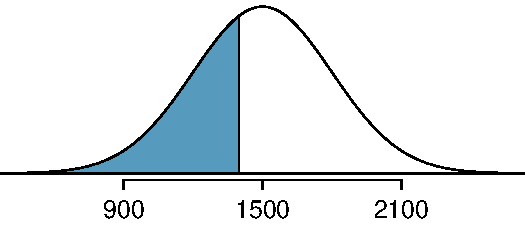
\includegraphics[height=22mm]{02/figures/satBelow1400/satBelow1400}
\end{center}
Identifying the mean $\mu=1500$, the standard deviation $\sigma=300$, and the cutoff for the tail area $x=1400$ makes it easy to compute the Z score:
\begin{eqnarray*}
Z = \frac{x - \mu}{\sigma} = \frac{1400 - 1500}{300} = -0.33
\end{eqnarray*}
Using the normal probability table, identify the row of $-0.3$ and column of $0.03$, which corresponds to the probability $0.3707$. Edward is at the $37^{th}$ percentile.
\end{example}

\begin{exercise}
Use the results of Example~\ref{edwardSatBelow1400} to compute the proportion of SAT takers who did better than Edward. Also draw a new picture.\footnote{If Edward did better than 37\% of SAT takers, then about 63\% must have done better than him. \\
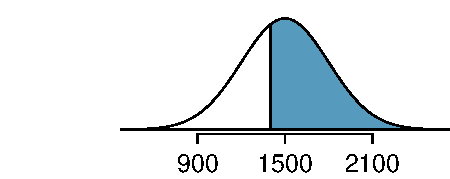
\includegraphics[height=12mm]{02/figures/satBelow1400/satAbove1400}}
\end{exercise}

\begin{tipBox}{\tipBoxTitle{areas to the right}
The normal probability table in most books gives the area to the left. If you would like the area to the right, first find the area to the left and then subtract this amount from~one.}
\end{tipBox}

\begin{exercise}
Stuart earned an SAT score of 2100. Draw a picture for each part. (a)~What is his percentile? (b)~What percent of SAT takers did better than Stuart?\footnote{Numerical answers: (a) 0.9772. (b) 0.0228.}
\end{exercise}

Based on a sample of 100 men,\footnote{This sample was taken from the USDA Food Commodity Intake Database.} the heights of male adults between the ages 20 and 62 in the US is nearly normal with mean 70.0'' and standard deviation 3.3''.

\begin{exercise}
Mike is 5'7'' and Jim is 6'4''. (a) What is Mike's height percentile? (b) What is Jim's height percentile? Also draw one picture for each part.\footnote{First put the heights into inches: 67 and 76 inches. Figures are shown below. (a) $Z_{Mike} = \frac{67 - 70}{3.3} = -0.91\ \to\ 0.1814$. (b) $Z_{Jim} = \frac{76 - 70}{3.3} = 1.82\ \to\ 0.9656$. \\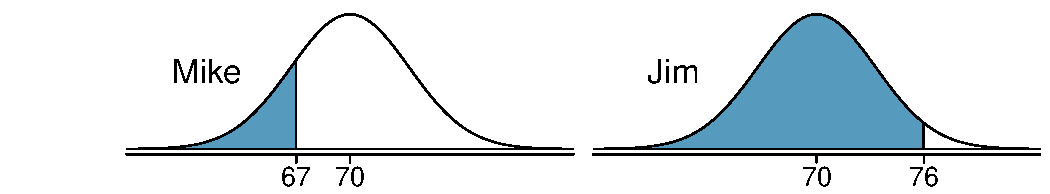
\includegraphics[height=12mm]{02/figures/mikeAndJimPercentiles/mikeAndJimPercentiles}}
\end{exercise}

The last several problems have focused on finding the probability or percentile for a particular observation. What if you would like to know the observation corresponding to a particular percentile?

\begin{example}{Erik's height is at the $40^{th}$ percentile. How tall is he?}\label{normalExam40Perc}
As always, first draw the picture.\vspace{-1mm}
\begin{center}
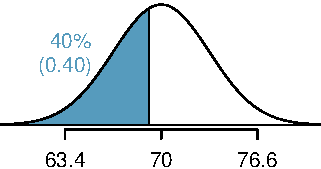
\includegraphics[height=22mm]{02/figures/height40Perc/height40Perc}\vspace{-1mm}
\end{center}
In this case, the lower tail probability is known (0.40), which can be shaded on the diagram. We want to find the observation that corresponds to this value. As a first step in this direction, we determine the Z score associated with the $40^{th}$ percentile.

Because the percentile is below 50\%, we know $Z$ will be negative. Looking in the negative part of the normal probability table, we search for the probability \emph{inside} the table closest to 0.4000. We find that 0.4000 falls in row $-0.2$ and between columns $0.05$ and $0.06$. Since it falls closer to $0.05$, we take this one: $Z=-0.25$.

Knowing $Z_{Erik}=-0.25$ and the population parameters $\mu=70$ and $\sigma=3.3$ inches, the Z score formula can be set up to determine Erik's unknown height, labeled $x_{Erik}$:
\begin{eqnarray*}
-0.25 = Z_{Erik} = \frac{x_{Erik} - \mu}{\sigma} = \frac{x_{Erik} - 70}{3.3}
\end{eqnarray*}
Solving for $x_{Erik}$ yields the height 69.18 inches. That is, Erik is about 5'9'' (this is notation for 5-feet, 9-inches).
\end{example}

\begin{example}{What is the adult male height at the $82^{nd}$ percentile?}
Again, we draw the figure first.\vspace{-1mm}
\begin{center}
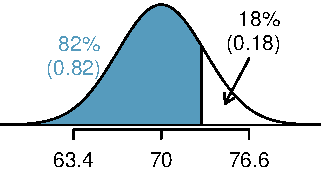
\includegraphics[height=22mm]{02/figures/height82Perc/height82Perc}\vspace{-1mm}
\end{center}
Next, we want to find the Z score at the $82^{nd}$ percentile, which will be a positive value. Looking in the Z table, we find $Z$ falls in row $0.9$ and the nearest column is $0.02$, i.e. $Z=0.92$. Finally, the height $x$ is found using the Z score formula with the known mean $\mu$, standard deviation $\sigma$, and Z score $Z=0.92$:
\begin{eqnarray*}
0.92 = Z = \frac{x-\mu}{\sigma} = \frac{x - 70}{3.3}
\end{eqnarray*}
This yields 73.04 inches or about 6'1'' as the height at the $82^{nd}$ percentile.
\end{example}

\begin{exercise}
(a) What is the $95^{th}$ percentile for SAT scores? (b) What is the $97.5^{th}$ percentile of the male heights? As always with normal probability problems, first draw a picture.\footnote{Remember: draw a picture first, then find the Z score. (We leave the pictures to you.) The Z score can be found by using the percentiles and the normal probability table. (a) We look for 0.95 in the probability portion (middle part) of the normal probability table, which leads us to row 1.6 and (about) column 0.05, i.e. $Z_{95}=1.65$. Knowing $Z_{95}=1.65$, $\mu = 1500$, and $\sigma = 300$, we setup the Z score formula: $1.65 = \frac{x_{95} - 1500}{300}$. We solve for $x_{95}$: $x_{95} = 1995$. (b) Similarly, we find $Z_{97.5} = 1.96$, again setup the Z score formula for the heights, and calculate $x_{97.5} = 76.5$.}
\end{exercise}

\begin{exercise}\label{more74Less69}
(a)~What is the probability that a randomly selected male adult is at least 6'2'' (74 inches)? (b)~What is the probability that a male adult is shorter than 5'9'' (69 inches)?\footnote{Numerical answers: (a) 0.1131. (b) 0.3821.}
\end{exercise}

\begin{example}{What is the probability that a random adult male is between 5'9'' and 6'2''?}
These heights correspond to 69 inches and 74 inches. First, draw the figure. The area of interest is no longer an upper or lower tail.
\begin{center}
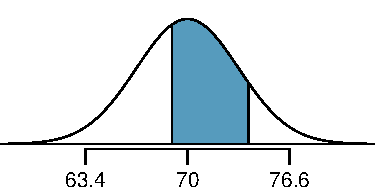
\includegraphics[height=0.85in]{02/figures/between59And62/between59And62}
\end{center}
The total area under the curve is~1. If we find the area of the two tails that are not shaded (from Exercise~\ref{more74Less69}, these areas are $0.3821$ and $0.1131$), then we can find the middle area:
\begin{center}
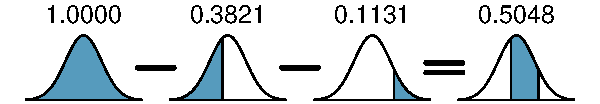
\includegraphics[height=0.65in]{02/figures/subtracting2Areas/subtracting2Areas}
\end{center}
That is, the probability of being between 5'9'' and 6'2'' is 0.5048.
\end{example}

\begin{exercise}
What percent of SAT takers get between 1500 and 2000?\footnote{This is an abbreviated solution. (Be sure to draw a figure!) First find the percent who get below 1500 and the percent that get above 2000: $Z_{1500} = 0.00 \to 0.5000$ (area below), $Z_{2000} = 1.67 \to 0.0475$ (area above). Final answer: $1.0000-0.5000 - 0.0475 = 0.4525$.}
\end{exercise}

\begin{exercise}
What percent of adult males are between 5'5'' and 5'7''?\footnote{5'5'' is 65 inches. 5'7'' is 67 inches. Numerical solution: $1.000 - 0.0649 - 0.8183 = 0.1168$, i.e. 11.68\%.}
\end{exercise}


\subsection{68-95-99.7 rule}

Here, we present a useful rule of thumb for the probability of falling within 1, 2, and 3 standard deviations of the mean in the normal distribution. This will be useful in a wide range of practical settings, especially when trying to make a quick estimate without a calculator or Z table.

\begin{figure}[hht]
\centering
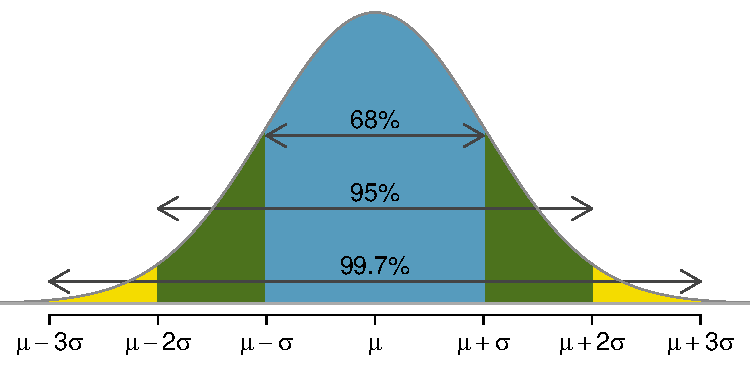
\includegraphics[height=1.9in]{02/figures/6895997/6895997}
\caption{Probabilities for falling within 1, 2, and 3 standard deviations of the mean in a normal distribution.}
\label{6895997}
\end{figure}

\begin{exercise}
Use the Z table to confirm that about 68\%, 95\%, and 99.7\% of observations fall within 1, 2, and 3, standard deviations of the mean in the normal distribution, respectively. For instance, first find the area that falls between $Z=-1$ and $Z=1$, which should have an area of about 0.68. Similarly there should be an area of about 0.95 between $Z=-2$ and $Z=2$.\footnote{First draw the pictures. To find the area between $Z=-1$ and $Z=1$, use the normal probability table to determine the areas below $Z=-1$ and above $Z=1$. Next verify the area between $Z=-1$ and $Z=1$ is about 0.68. Repeat this for $Z=-2$ to $Z=2$ and also for $Z=-3$ to $Z=3$.}
\end{exercise}

It is possible for a normal random variable to fall 4,~5, or~even more standard deviations from the mean. However, these occurrences are very rare if the data are nearly normal. The probability of being further than 4 standard deviations from the mean is about 1-in-30,000. For 5 and 6 standard deviations, it is about 1-in-3.5 million and 1-in-1 billion, respectively.

\begin{exercise}
SAT scores closely follow the normal model with mean $\mu = 1500$ and standard deviation $\sigma = 300$. (a) About what percent of test takers score 900 to 2100? (b) What percent score between 1500 and 2100?\footnote{(a) 900 and 2100 represent two standard deviations above and below the mean, which means about 95\% of test takers will score between 900 and 2100. (b)~Since the normal model is symmetric, then half of the test takers from part~(a) ($\frac{95\%}{2} = 47.5\%$ of all test takers) will score 900 to 1500 while 47.5\% score between 1500 and 2100.}
\end{exercise}


\subsection{Evaluating the normal approximation}
\label{assessingNormal}

Many processes can be well approximated by the normal distribution. We have already seen two good examples: SAT scores and the heights of US adult males. While using a normal model can be extremely convenient and helpful, it is important to remember normality is always an approximation. Testing the appropriateness of the normal assumption is a key step in many data analyses.

Example~\ref{normalExam40Perc} suggests the distribution of heights of US males is well approximated by the normal model. We are interested in proceeding under the assumption that the data are normally distributed, but first we must check to see if this is reasonable.

There are two visual methods for checking the assumption of normality, which can be implemented and interpreted quickly. The first is a simple histogram with the best fitting normal curve overlaid on the plot, as shown in the left panel of Figure~\ref{fcidMHeights}. The sample mean $\bar{x}$ and standard deviation $s$ are used as the parameters of the best fitting normal curve. The closer this curve fits the histogram, the more reasonable the normal model assumption. Another more common method is examining a \term{normal probability plot}.\footnote{Also commonly called a \term{quantile-quantile plot}.}, shown in the right panel of Figure~\ref{fcidMHeights}. The closer the points are to a perfect straight line, the more confident we can be that the data follow the normal model.

\begin{figure}
\centering
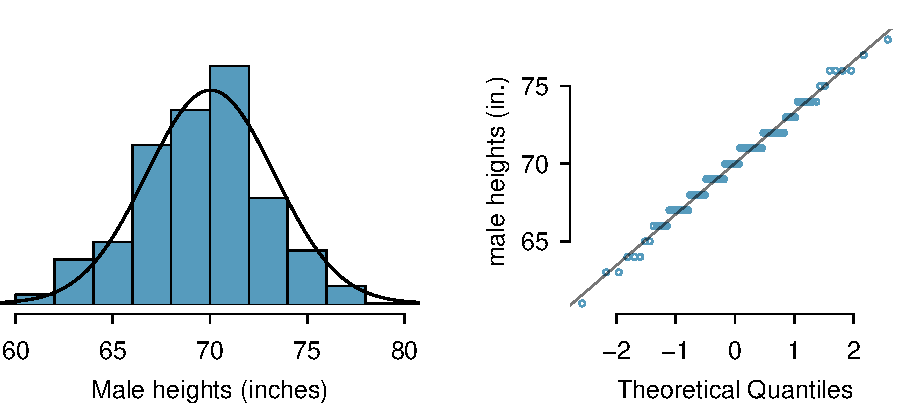
\includegraphics[width=0.8\textwidth]{02/figures/fcidMHeights/fcidMHeights}
\caption{A sample of 100 male heights. The observations are rounded to the nearest whole inch, explaining why the points appear to jump in increments in the normal probability plot.}
\label{fcidMHeights}
\end{figure}

\begin{example}{Three data sets of 40, 100, and 400 samples were simulated from a normal distribution, and the histograms and normal probability plots of the data sets are shown in Figure~\ref{normalExamples}. These will provide a benchmark for what to look for in plots of real data.} \label{normalExamplesExample}

\begin{figure}
\centering
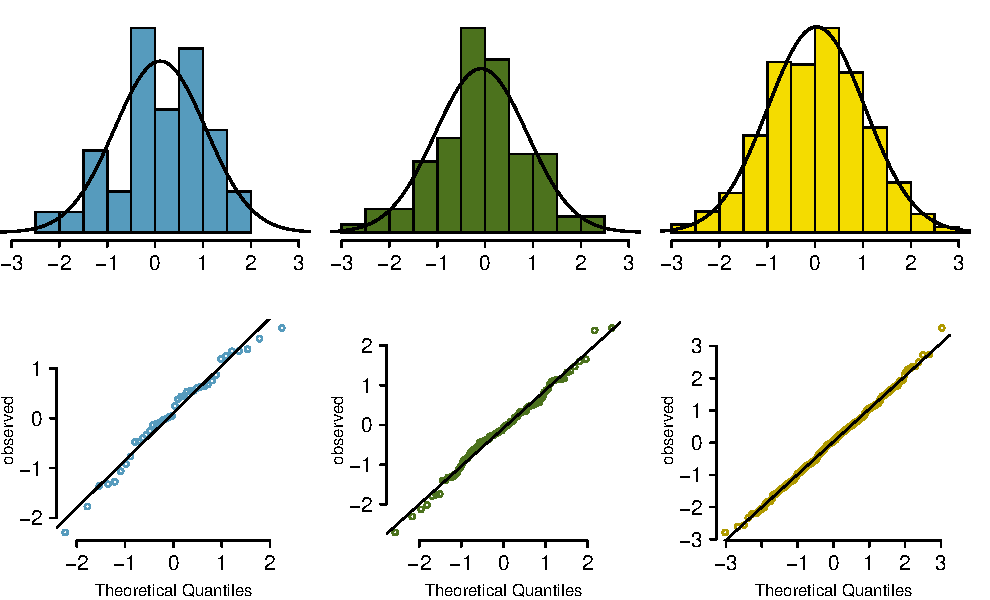
\includegraphics[width=\textwidth]{02/figures/normalExamples/normalExamples}
\caption{Histograms and normal probability plots for three simulated normal data sets; $n=40$ (left), $n=100$ (middle), $n=400$ (right).}
\label{normalExamples}
\end{figure}

The left panels show the histogram (top) and normal probability plot (bottom) for the simulated data set with 40 observations. The data set is too small to really see clear structure in the histogram. The normal probability plot also reflects this, where there are some deviations from the line. However, these deviations are not strong.

The middle panels show diagnostic plots for the data set with 100 simulated observations. The histogram shows more normality and the normal probability plot shows a better fit. While there is one observation that deviates noticeably from the line, it is not particularly extreme.

The data set with 400 observations has a histogram that greatly resembles the normal distribution, while the normal probability plot is nearly a perfect straight line. Again in the normal probability plot there is one observation (the largest) that deviates slightly from the line. If that observation had deviated 3 times further from the line, it would be of much greater concern in a real data set. Apparent outliers can occur in normally distributed data but they are rare.

Notice the histograms look more normal as the sample size increases, and the normal probability plot becomes straighter and more stable.
\end{example}

\begin{example}{Are NBA player heights normally distributed? Consider all 435 NBA players from the 2008-9 season presented in Figure~\ref{nbaNormal}.\footnote{These data were collected from \urlwofont{http://www.nba.com}.}}
We first create a histogram and normal probability plot of the NBA player heights. The histogram in the left panel is slightly left skewed, which contrasts with the symmetric normal distribution. The points in the normal probability plot do not appear to closely follow a straight line but show what appears to be a ``wave''. We can compare these characteristics to the sample of 400 normally distributed observations in Example~\ref{normalExamplesExample} and see that they represent much stronger deviations from the normal model. NBA player heights do not appear to come from a normal distribution.
\end{example}

\begin{figure}
\centering
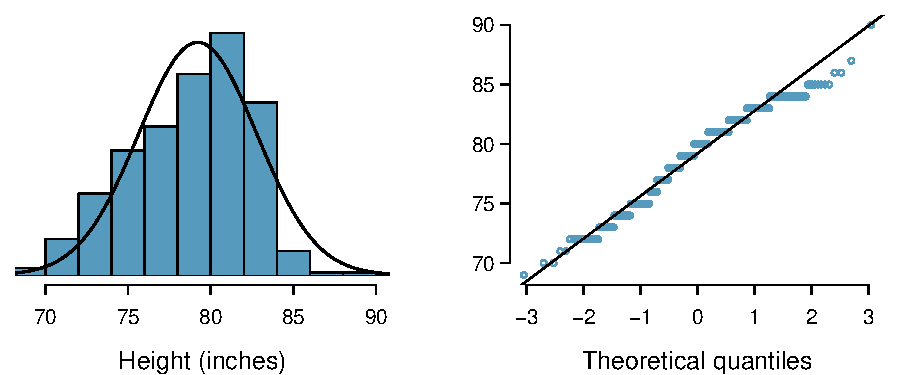
\includegraphics[width=\textwidth]{02/figures/nbaNormal/nbaNormal}
\caption{Histogram and normal probability plot for the NBA heights from the 2008-9 season.}
\label{nbaNormal}
\end{figure}

\begin{example}{Can we approximate poker winnings by a normal distribution? We consider the poker winnings of an individual over 50 days. A histogram and normal probability plot of these data are shown in Figure~\ref{pokerNormal}.}
The data are very strongly right skewed\index{skew!example: very strong} in the histogram, which corresponds to the very strong deviations on the upper right component of the normal probability plot. If we compare these results to the sample of 40 normal observations in Example~\ref{normalExamplesExample}, it is apparent that these data show very strong deviations from the normal model.
\end{example}

\begin{figure}
\centering
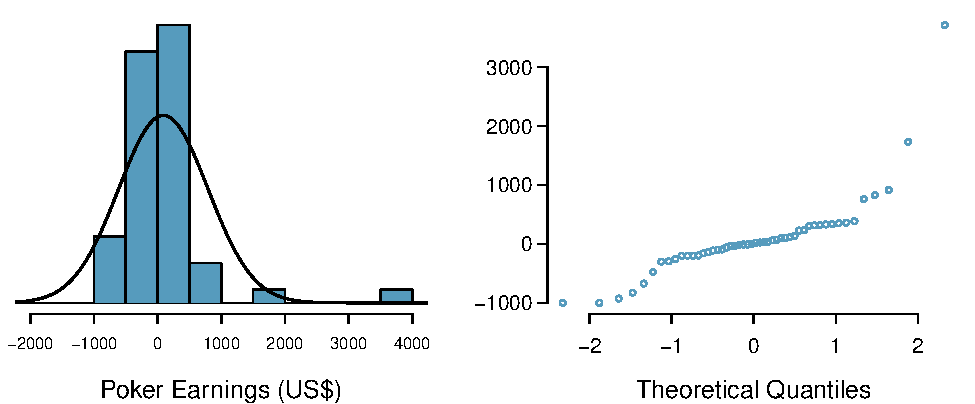
\includegraphics[width=\textwidth]{02/figures/pokerNormal/pokerNormal}
\caption{A histogram of poker data with the best fitting normal plot and a normal probability plot.}
\label{pokerNormal}
\end{figure}

\begin{exercise}\label{normalQuantileExercise}
Determine which data sets represented in Figure~\ref{normalQuantileExer} plausibly come from a nearly normal distribution. Are you confident in all of your conclusions? There are 100 (top left), 50 (top right), 500 (bottom left), and 15 points (bottom right) in the four plots.\footnote{Answers may vary a little. The top-left plot shows some deviations in the smallest values in the data set; specifically, the left tail of the data set has some outliers we should be wary of. The top-right and bottom-left plots do not show any obvious or extreme deviations from the lines for their respective sample sizes, so a normal model would be reasonable for these data sets. The bottom-right plot has a consistent curvature that suggests it is not from the normal distribution. If we examine just the vertical coordinates of these observations, we see that there is a lot of data between -20 and 0, and then about five observations scattered between 0 and 70. This describes a distribution that has a strong right skew.}
\end{exercise}

\begin{figure}
\centering
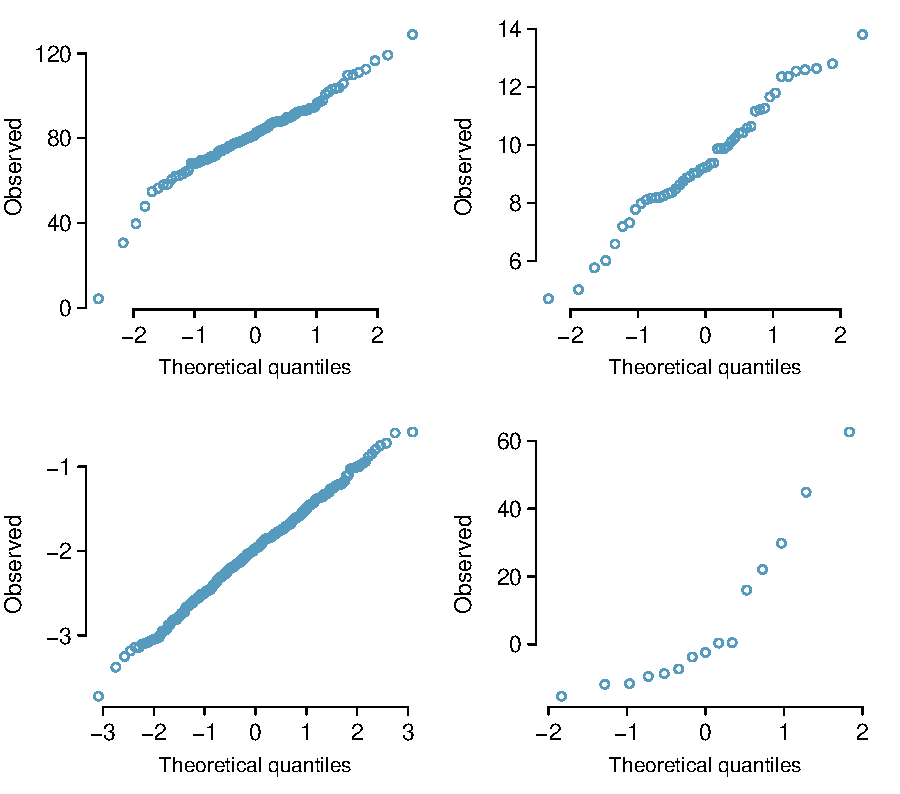
\includegraphics[width=0.9\textwidth]{02/figures/normalQuantileExer/normalQuantileExer}
\caption{Four normal probability plots for Exercise~\ref{normalQuantileExercise}.}
\label{normalQuantileExer}
\end{figure}

\begin{exercise} \label{normalQuantileExerciseAdditional}
Figure~\ref{normalQuantileExerAdditional} shows normal probability plots for two distributions that are skewed. One distribution is skewed to the low end (left skewed) and the other to the high end (right skewed). Which is which?\footnote{Examine where the points fall along the vertical axis. In the first plot, most points are near the low end with fewer observations scattered along the high end; this describes a distribution that is skewed to the high end. The second plot shows the opposite features, and this distribution is skewed to the low end.}
\index{normal distribution|)}
\end{exercise}

\begin{figure}
\centering
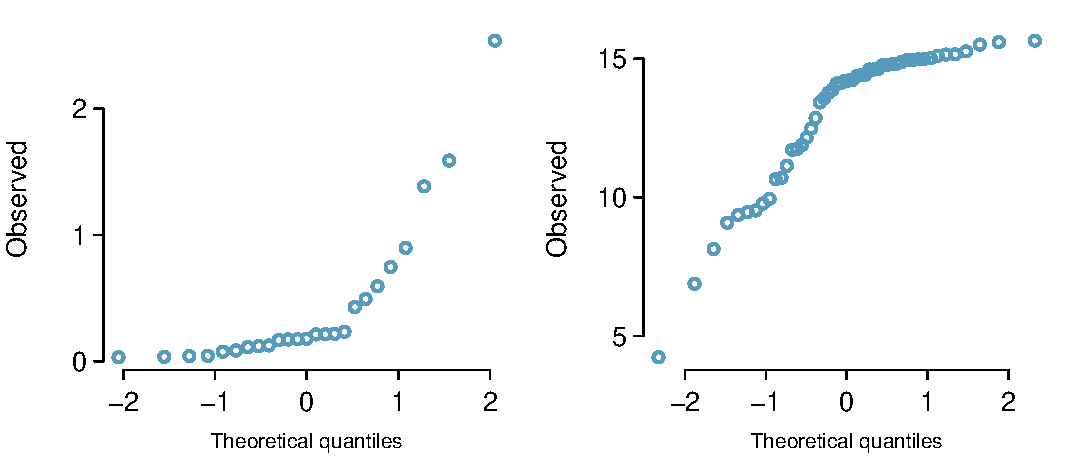
\includegraphics[width=0.9\textwidth]{02/figures/normalQuantileExer/normalQuantileExerAdditional}
\caption{Normal probability plots for Exercise~\ref{normalQuantileExerciseAdditional}.}
\label{normalQuantileExerAdditional}
\end{figure}


%_________________
\section{Applying the normal model}
\label{ApplyingTheNormalModel}

The approach for using the normal model in the context of inference is very similar to the practice of applying the model to individual observations that are nearly normal. We will replace null distributions we previously obtained using the randomization or simulation techniques and verify the results once again using the normal model. When the sample size is sufficiently large, this approximation generally provides us with the same conclusions.

\subsection{Standard error}

Point estimates vary from sample to sample, and we quantify this variability with what is called the \term{standard error (SE)}. The standard error is equal to the standard deviation associated with the estimate. So, for example, if we used the standard deviation to quantify the variability of a point estimate from one sample to the next, this standard deviation would be called the standard error of the point estimate.

% The large the sample size, the smaller our standard error a statistic like the sample proportion or sample mean will b smaller. This is consistent with intuition: the more data we have, the more accurate an estimate will tend to be, i.e.~the standard error of the estimate becomes smaller when we have more data.

The way we determine the standard error varies from one situation to the next. However, typically it is determined using a formula based on the Central Limit Theorem.


\subsection{Normal model application: opportunity cost}

In Section~\ref{caseStudyOpportunityCost} we were introduced to the opportunity cost study, which found that students became thriftier when they were reminded that not spending money now means the money can be spent on other things in the future. Let's re-analyze the data in the context of the normal distribution and compare the results.

Figure~\ref{OpportunityCostDiffs_w_normal} summarizes the null distribution as determined using the randomization method. The best fitting normal distribution for the null distribution has a mean of 0. We can calculate the standard error of this distribution by borrowing a formula that we will become familiar with in Section~\ref{differenceOfTwoProportions}, but for now let's just take the value $SE = 0.078$ as a~given. Recall that the point estimate of the difference was 0.20, as shown in the plot. Next, we'll use the normal distribution approach to compute the two-tailed p-value.

\begin{figure}
\centering
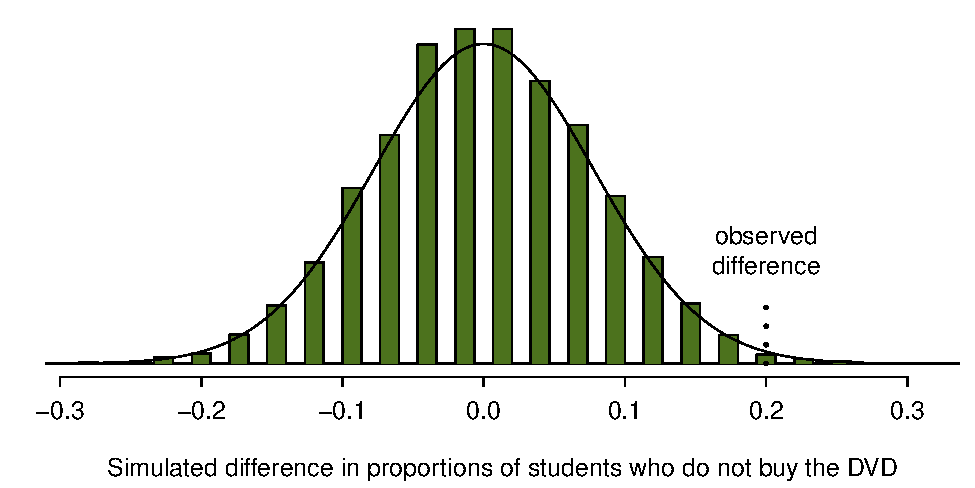
\includegraphics[width=0.85\textwidth]{02/figures/OpportunityCost/OpportunityCostDiffs_w_normal}
\caption{Null distribution of differences with an overlaid normal curve for the opportunity cost study.}
\label{OpportunityCostDiffs_w_normal}
\end{figure}

As we learned in Section~\ref{normalDist}, it is helpful to draw and shade a picture of the normal distribution so we know precisely what we want to calculate. Here we want to find the area of the two tails representing the p-value.
\begin{center}
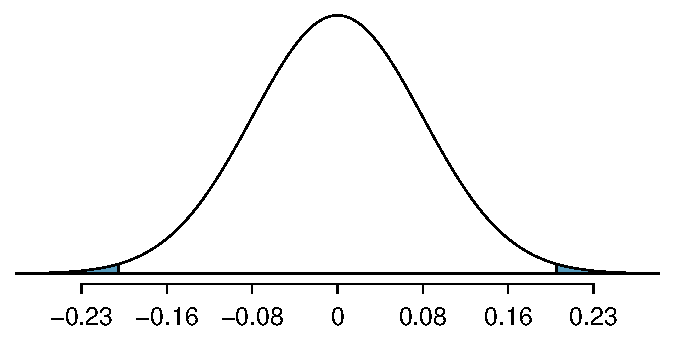
\includegraphics[width=0.5\textwidth]{02/figures/OpportunityCost/OpportunityCostDiffs_normal_only}
\end{center}
Next, we can calculate the Z score using the observed difference, 0.20, and the two model parameters. The standard error, $SE = 0.078$, is the equivalent of the model's standard deviation.
\begin{align*}
Z = \frac{\text{observed difference} - 0}{SE} = \frac{0.20 - 0}{0.078} = 2.56
\end{align*}
We can either look up $Z = 2.56$ in the normal probability table or use statistical software to determine the right tail area: 0.0052, which is about the same as what we got for the right tail using the randomization approach (0.0065). Doubling this value yields the total area in the two tails and the p-value for the hypothesis test: 0.01. As before, since the p-value is less than 0.05, we conclude that the treatment did indeed impact students' spending.

\begin{termBox}{\tBoxTitle{Z score in a hypothesis test}
In the context of a hypothesis test, the Z score for a point estimate is
\begin{align*}
Z = \frac{\text{point estimate} - \text{null value}}{SE}
\end{align*}
The standard error in this case is the equivalent of the standard deviation of the point estimate, and the null value comes from the null hypothesis.}
\end{termBox}

We have confirmed that the randomization approach we used earlier and the normal distribution approach provide almost identical p-values and conclusions in the opportunity cost case study. Next, let's turn our attention to the medical consultant case study.


\subsection{Normal model application: medical consultant}

In Section~\ref{SimulationCaseStudies} we learned about a medical consultant who reported that only 3 of her 62 clients who underwent a liver transplant had complications, which is less than the more common complication rate of 0.10. As in the other case studies, we identified a suitable null distribution using a simulation approach, as shown in Figure~\ref{MedConsNullSim_w_normal}. Here we have added the best-fitting normal curve to the figure, which has a mean of 0.10. Borrowing a formula that we'll encounter in Chapter~\ref{inferenceForCategoricalData}, the standard error of this distribution was also computed: $SE = 0.038$.
%\begin{align*}
%SE = \sqrt{\frac{p_0 (1 - p_0)}{n}} = \sqrt{\frac{0.1 (1 - 0.1)}{62}} = 0.038
%\end{align*}
%where $p_0$ is the null value for the hypothesis test and $n$ is the sample size. (We'll discuss this formula in greater detail in next chapter.) 

In the previous analysis, we obtained a p-value of 0.2444, and we will try to reproduce that p-value using the normal distribution approach. However, before we begin, we want to point out a simple detail that is easy to overlook: the null distribution we earlier generated is slightly skewed, and the distribution isn't that smooth. In fact, the normal distribution only sort-of fits this model. We'll discuss this discrepancy more in a moment.

\begin{figure}
\centering
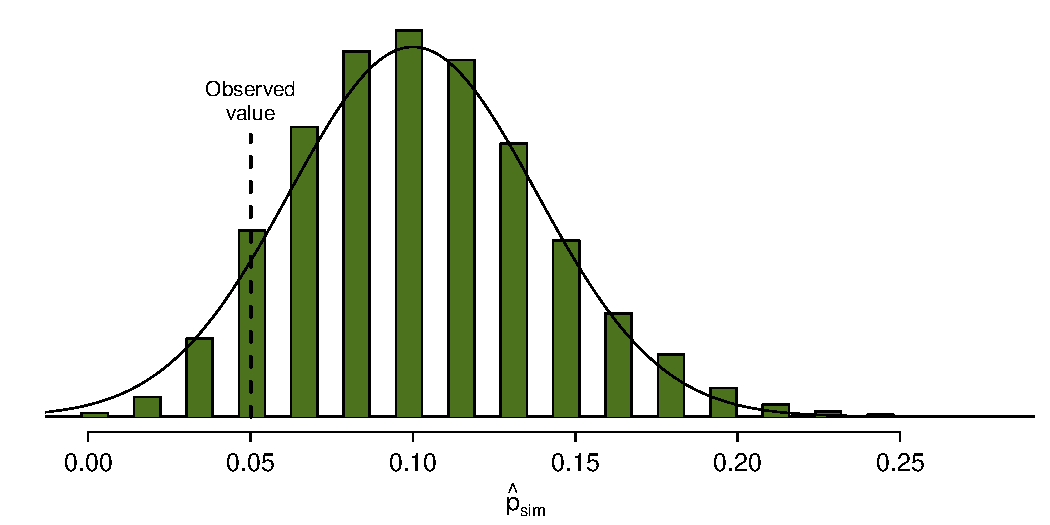
\includegraphics[width=0.8\textwidth]{02/figures/MedicalConsultant/MedConsNullSim_w_normal}
\caption{The null distribution for $\hat{p}$, created from 10,000 simulated studies, along with the best-fitting normal model.}
\label{MedConsNullSim_w_normal}
\end{figure}

We'll again begin by creating a picture. Here a normal distribution centered at 0.10 with a standard error of 0.038.
\begin{center}
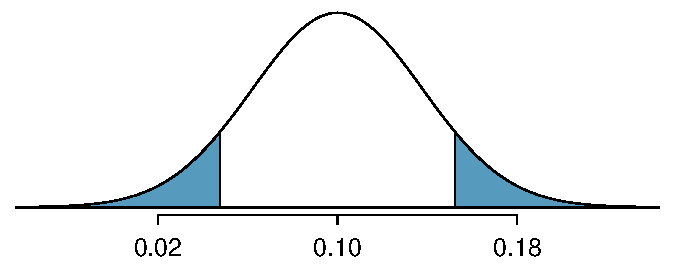
\includegraphics[width=0.4\textwidth]{02/figures/MedicalConsultant/MedConsNullSim_normal_only}
\end{center}
Next, we can calculate the Z score using the observed complication rate, $\hat{p} = 0.048$ along with the mean and standard deviation of the normal model. Here again, we use the standard error for the standard deviation.
\begin{align*}
Z = \frac{\hat{p} - p_0}{SE_{\hat{p}}} = \frac{0.048 - 0.10}{0.038} = -1.37
\end{align*}
Identifying $Z = -1.37$ in the normal probability table or using statistical software, we can determine that the left tail area is 0.0853. Doubling this value yields the total area in the two tails: about 0.17. This is the estimated p-value for the hypothesis test. However, there's a problem: this is very different than the earlier p-value we computed: 0.2444.

The discrepancy is explained by normal model's poor representation of the null distribution in Figure~\ref{MedConsNullSim_w_normal}. As noted earlier, the null distribution from the simulations is not very smooth, and the distribution itself is slightly skewed. That's the bad news. The good news is that typically we can foresee these problems using some simple checks (we'll see these later).

In Section~\ref{CLTsection} we noted that the two common requirements for the Central Limit Theorem to apply are that (1) the observations in the sample must be independent, and (2) the sample must be sufficiently large. The guidelines for this particular situation -- which we will learn in Section~\ref{singleProportion} -- would have alerted us that the normal model was a poor approximation.


\subsection{Conditions for applying the normal model}

The success story in this section was the application of the normal model in the context of the opportunity cost data. However, the biggest lesson comes from our failed attempt to use the normal approximation in the medical consultant case study.

Statistical techniques are like a carpenter's tools. When used responsibly, they can produce amazing and precise results. However, if the tools are applied irresponsibly or under inappropriate conditions, they will produce unreliable results. For this reason, with every statistical method that we introduce in future chapters, we will carefully outline conditions when the method can reasonably be used. These conditions should be checked in each application of the technique.


%_________________
\section{Confidence intervals}
\label{ConfidenceIntervals}

\index{confidence interval|(}

A point estimate provides a single plausible value for a parameter. However, a point estimate is rarely perfect; usually there is some error in the estimate. Instead of supplying just a point estimate of a parameter, a next logical step would be to provide a plausible \emph{range of values} for the parameter.


\subsection{Capturing the population parameter}

A plausible range of values for the population parameter is called a \term{confidence interval}. Using only a point estimate is like fishing in a murky lake with a spear, and using a confidence interval is like fishing with a net. We can throw a spear where we saw a fish, but we will probably miss. On the other hand, if we toss a net in that area, we have a good chance of catching the fish.

If we report a point estimate, we probably will not hit the exact population parameter. On the other hand, if we report a range of plausible values -- a confidence interval -- we have a good shot at capturing the parameter.

\begin{exercise}
If we want to be very certain we capture the population parameter, should we use a wider interval or a smaller interval?\footnote{If we want to be more certain we will capture the fish, we might use a wider net. Likewise, we use a wider confidence interval if we want to be more certain that we capture the parameter.}
\end{exercise}


\subsection{Constructing a 95\% confidence interval}

A point estimate is our best guess for the value of the parameter, so it makes sense to build the confidence interval around that value. The standard error, which is a measure of the uncertainty associated with the point estimate, provides a guide for how large we should make the confidence interval.

\begin{termBox}{\tBoxTitle{Constructing a 95\% confidence interval}
When the sampling distribution of a point estimate can reasonably be modeled as normal, the point estimate we observe will be within 1.96 standard errors of the true value of interest about 95\% of the time. Thus, a \term{95\% confidence interval} for such a point estimate can be constructed:\vspace{-2mm}
\begin{align}
\text{point estimate}\ \pm\ 1.96 \times SE\vspace{-1mm}
\label{95PercentConfidenceIntervalFormula}
\end{align}
We can be \termsub{95\% confident}{confident} this interval captures the true value.}
\end{termBox}

\begin{exercise}
Compute the area between -1.96 and 1.96 for a normal distribution with mean 0 and standard deviation 1.~\footnote{We will leave it to you to draw a picture. The Z scores are $Z_{left} = -1.96$ and $Z_{right} = 1.96$. The area between these two Z scores is $0.9750 - 0.0250 = 0.9500$. This is where ``1.96'' comes from in the 95\% confidence interval formula.}
\end{exercise}

\begin{example}{The point estimate from the opportunity cost study was that 20\% fewer students would buy a DVD if they were reminded that money not spent now could be spent later on something else. The point estimate from this study can reasonably be modeled with a normal distribution, and a proper standard error for this point estimate is $SE = 0.078$. Construct a 95\% confidence interval.\footnote{We've used $SE = 0.078$ from the last section. However, it would more generally be appropriate to recompute the $SE$ slightly differently for this confidence interval using the technique introduced in Section~\ref{SampleDistributionOfTheDiffOfTwoProportions}. Don't worry about this detail for now since the two resulting standard errors are, in this case, almost identical.}}
% Using the old SE intentionally to keep things consistent / simple.
% Correct SE: p1 <- 56 / 75; p2 <- 41 / 75; sqrt(p1 * (1 - p1) / 75 + p2 * (1 - p2) / 75)
Since the conditions for the normal approximation have already been verified, we can move forward with the construction of the 95\% confidence interval:
\begin{align*}
\text{point estimate}\ \pm\ 1.96 \times SE \quad \rightarrow \quad
0.20\ \pm\ 1.96 \times 0.078 \quad \rightarrow \quad
(0.047, 0.353)
\end{align*}
We are 95\% confident that the DVD purchase rate resulting from the treatment is between 4.7\% and 35.3\% lower than in the control group. Since this confidence interval does not contain 0, it is consistent with our earlier result where we rejected the notion of ``no difference'' using a hypothesis test.
\end{example}

\begin{example}{In Section~\ref{basicExampleOfStentsAndStrokes} we encountered an experiment that examined whether implanting a stent in the brain of a patient at risk for a stroke helps reduce the risk of a stroke. The results from the first 30 days of this study, which included 451 patients, are summarized in Table~\ref{stentStudyResultsCIsection}. These results are surprising! The point estimate suggests that patients who received stents may have a \emph{higher} risk of stroke: $p_{trmt} - p_{ctrl} = 0.090$. The conditions necessary to ensure the point estimate is nearly normal have been verified for you, and the estimate's standard error is $SE = 0.028$. Construct a 95\% confidence interval for the change in 30-day stroke rates from usage of the stent.}
\label{stentStroke95CI_CIsection}
The conditions for applying the normal model have already been verified, so we can proceed to the construction of the confidence interval:
\begin{align*}
\text{point estimate}\ \pm\ 1.96 \times SE \quad \rightarrow \quad
0.090\ \pm\ 1.96 \times 0.028 \quad \rightarrow \quad
(0.035, 0.145)
\end{align*}
We are 95\% confident that implanting a stent in a stroke patient's brain increased the risk of stroke within 30 days by a rate of 0.035 to 0.145. This confidence interval can also be used in a way analogous to a hypothesis test: since the interval does not contain 0, it means the data provide statistically significant evidence that the stent used in the study \emph{increases} the risk of stroke, contrary to what researchers had expected before this study was published!
\end{example}

\begin{table}[h]
\centering
\begin{tabular}{l cc c}
  \hline
	& 	stroke 	& no event & Total \\
  \hline
treatment 	& 33		& 191	& 224 \\
control 	& 13		& 214	& 227 \\
  \hline
Total		& 46		& 405	& 451 \\
  \hline
\end{tabular}
\caption{Descriptive statistics for 30-day results for the stent study.}
\label{stentStudyResultsCIsection}
\end{table}

As with hypothesis tests, confidence intervals are imperfect. About 1-in-20 properly constructed confidence intervals will fail to capture the parameter of interest. Figure~\ref{95PercentConfidenceInterval} shows 25 confidence intervals for a proportion that were constructed from simulations where the true proportion was $p = 0.3$. However, 1 of these 25 confidence intervals happened not to include the true value.

\begin{figure}[hht]
   \centering
   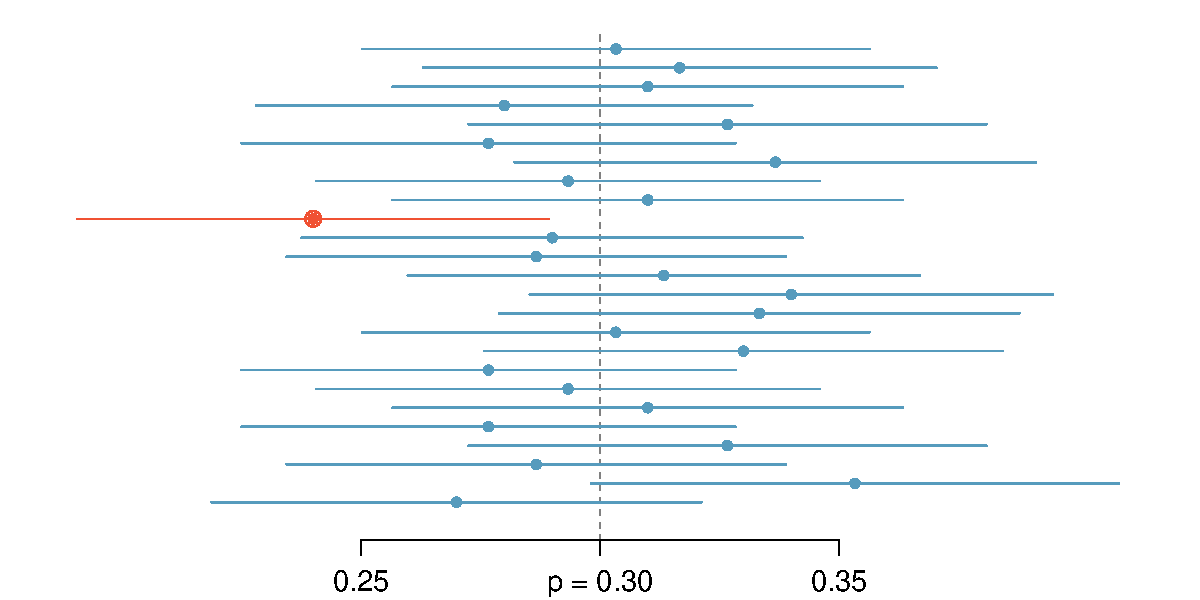
\includegraphics[width=\textwidth]{02/figures/95PercentConfidenceInterval/95PercentConfidenceInterval}
   \caption{Twenty-five samples of size $n=300$ were simulated when $p = 0.30$. For each sample, a confidence interval was created to try to capture the true proportion $p$. However,~1~of these~25 intervals did not capture $p = 0.30$.}
   \label{95PercentConfidenceInterval}
\end{figure}

\begin{exercise}
In Figure~\ref{95PercentConfidenceInterval}, one interval does not contain the true proportion, $p = 0.3$. Does this imply that there was a problem with the simulations run?\footnote{No. Just as some observations occur more than 1.96 standard deviations from the mean, some point estimates will be more than 1.96 standard errors from the parameter. A confidence interval only provides a plausible range of values for a parameter. While we might say other values are implausible based on the data, this does not mean they are impossible.}
\end{exercise}


\subsection{Changing the confidence level}
\label{changingTheConfidenceLevelSection}

\index{confidence interval!confidence level|(}

Suppose we want to consider confidence intervals where the confidence level is somewhat higher than 95\%: perhaps we would like a confidence level of 99\%. Think back to the analogy about trying to catch a fish: if we want to be more sure that we will catch the fish, we should use a wider net. To create a 99\% confidence level, we must also widen our 95\% interval. On the other hand, if we want an interval with lower confidence, such as 90\%, we could make our original 95\% interval slightly slimmer.

The 95\% confidence interval structure provides guidance in how to make intervals with new confidence levels. Below is a general 95\% confidence interval for a point estimate that comes from a nearly normal distribution:
\begin{eqnarray}
\text{point estimate}\ \pm\ 1.96\times SE
\end{eqnarray}
There are three components to this interval: the point estimate, ``1.96'', and the standard error. The choice of $1.96\times SE$ was based on capturing 95\% of the data since the estimate is within 1.96 standard errors of the true value about 95\% of the time. The choice of 1.96 corresponds to a 95\% confidence level. 

\begin{exercise} \label{leadInForMakingA99PercentCIExercise}
If $X$ is a normally distributed random variable, how often will $X$ be within 2.58 standard deviations of the mean?\footnote{This is equivalent to asking how often the $Z$ score will be larger than -2.58 but less than 2.58. (For a picture, see Figure~\ref{choosingZForCI}.) To determine this probability, look up -2.58 and 2.58 in the normal probability table (0.0049 and 0.9951). Thus, there is a $0.9951-0.0049 \approx 0.99$ probability that the unobserved random variable $X$ will be within 2.58 standard deviations of the mean.}
\end{exercise}

To create a 99\% confidence interval, change 1.96 in the 95\% confidence interval formula to be $2.58$. Exercise~\ref{leadInForMakingA99PercentCIExercise} highlights that 99\% of the time a normal random variable will be within 2.58 standard deviations of its mean. This approach -- using the Z scores in the normal model to compute confidence levels -- is appropriate when the point estimate is associated with a normal distribution and we can properly compute the standard error. Thus, the formula for a 99\% confidence interval is
\begin{eqnarray}
\text{point estimate}\ \pm\ 2.58\times SE
\label{99PercCIForMean}
\label{99PercCIForNormalPointEstimate}
\end{eqnarray}
%\Comment{I don't know where the equation number above gets referenced. Might drop the equation number.}

\begin{figure}[ht]
\centering
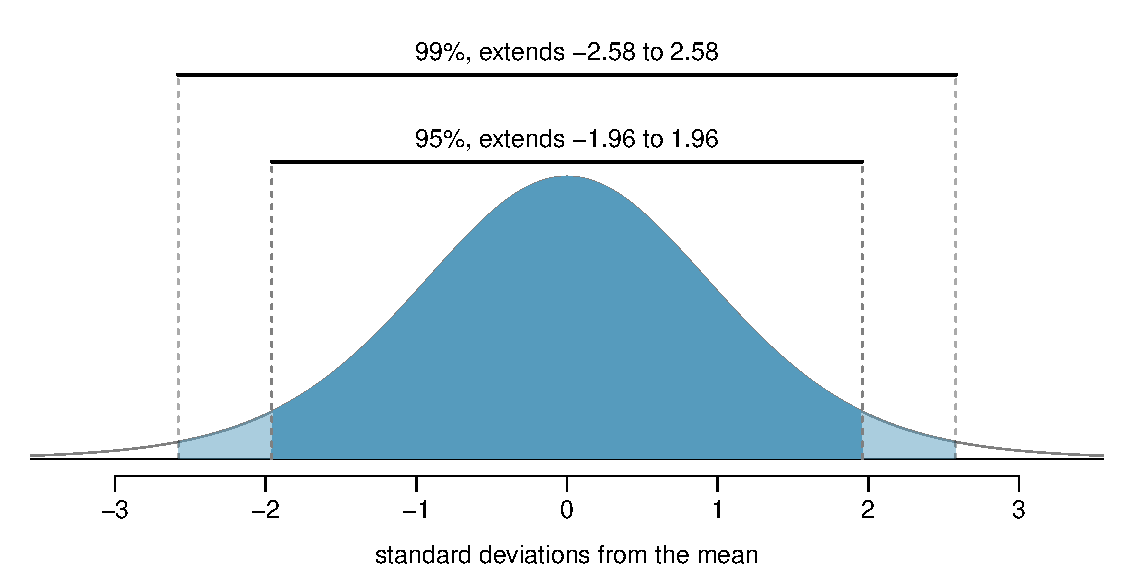
\includegraphics[width=\textwidth]{02/figures/choosingZForCI/choosingZForCI}
\caption{The area between -$z^{\star}$ and $z^{\star}$ increases as $|z^{\star}|$ becomes larger. If the confidence level is 99\%, we choose $z^{\star}$ such that 99\% of the normal curve is between -$z^{\star}$ and $z^{\star}$, which corresponds to 0.5\% in the lower tail and 0.5\% in the upper tail: $z^{\star}=2.58$.}
\label{choosingZForCI}
\index{confidence interval!confidence level|)}
\end{figure}

The normal approximation is crucial to the precision of these confidence intervals. The next two chapters provides detailed discussions about when the normal model can safely be applied to a variety of situations. When the normal model is not a good fit, we will use alternative distributions that better characterize the sampling distribution.

\Comment{Reminder for David: EOCE 4.9 (as of 2nd Edition) must now be changed since it relied on content that is now deleted.}

\begin{exercise} \label{find99CIForRun10AgeExercise}
Create a 99\% confidence interval for the impact of the stent on the risk of stroke using the data from Example~\ref{stentStroke95CI_CIsection}. The point estimate is 0.090, and the standard error is $SE = 0.028$. It has been verified for you that the point estimate can reasonably be modeled by a normal distribution.\footnote{Since the necessary conditions for applying the normal model have already been checked for us, we can go straight to the construction of the confidence interval: $\text{point estimate}\ \pm\ 2.58 \times  SE \rightarrow (0.018, 0.162)$. We are 99\% confident that implanting a stent in the brain of a patient who is at risk of stroke increases the risk of stroke within 30 days by a rate of 0.018 to 0.162.}
\end{exercise}

\begin{termBox}{\tBoxTitle{Confidence interval for any confidence level}
If the point estimate follows the normal model with standard error $SE$, then a confidence interval for the population parameter is
\begin{eqnarray*}
\text{point estimate}\ \pm\ z^{\star} SE
\end{eqnarray*}
where $z^{\star}$ corresponds to the confidence level selected.}
\end{termBox}

Figure~\ref{choosingZForCI} provides a picture of how to identify $z^{\star}$ based on a confidence level. We select $z^{\star}$ so that the area between -$z^{\star}$ and $z^{\star}$ in the normal model corresponds to the confidence level. 

\begin{termBox}{\tBoxTitle{Margin of error}
\label{marginOfErrorTermBox}In a confidence interval, $z^{\star}\times SE$ is called the \term{margin of error}.}
\end{termBox}

\begin{exercise} \label{find90CIForRun10AgeExercise}
In Example~\ref{stentStroke95CI_CIsection} we found that implanting a stent in the brain of a patient at risk for a stroke \emph{increased} the risk of a stroke. The study estimated a 9\% increase in the number of patients who had a stroke, and the standard error of this estimate was about $SE = 2.8\%$. Compute a 90\% confidence interval for the effect.\footnote{We must find $z^{\star}$ such that 90\% of the distribution falls between -$z^{\star}$ and $z^{\star}$ in the standard normal model, $N(\mu=0, \sigma=1)$. We can look up -$z^{\star}$ in the normal probability table by looking for a lower tail of 5\% (the other 5\% is in the upper tail), thus $z^{\star}=1.65$. The 90\% confidence interval can then be computed as $\text{point estimate}\ \pm\ 1.65\times SE \to (4.4\%, 13.6\%)$. (Note: the conditions for normality had earlier been confirmed for us.) That is, we are 90\% confident that implanting a stent in a stroke patient's brain increased the risk of stroke within 30 days by 4.4\% to 13.6\%.}
\end{exercise}

\subsection{Interpreting confidence intervals}
\label{interpretingCIs}

\index{confidence interval!interpretation|(}

A careful eye might have observed the somewhat awkward language used to describe confidence intervals. Correct interpretation:
\begin{quote}
We are XX\% confident that the population parameter is between...
\end{quote}
\emph{Incorrect} language might try to describe the confidence interval as capturing the population parameter with a certain probability. This is one of the most common errors: while it might be useful to think of it as a probability, the confidence level only quantifies how plausible it is that the parameter is in the interval.

Another especially important consideration of confidence intervals is that they \emph{only try to capture the population parameter}. Our intervals say nothing about the confidence of capturing individual observations, a proportion of the observations, or about capturing point estimates. Confidence intervals only attempt to capture population parameters.

\index{confidence interval!interpretation|)}
\index{confidence interval|)}



